\documentclass[11pt]{aghdpl}
% \documentclass[en,11pt]{aghdpl}  % praca w języku angielskim

% Lista wszystkich języków stanowiących języki pozycji bibliograficznych użytych w pracy.
% (Zgodnie z zasadami tworzenia bibliografii każda pozycja powinna zostać utworzona zgodnie z zasadami języka, w którym dana publikacja została napisana.)
\usepackage[english,polish]{babel}

% Użyj polskiego łamania wyrazów (zamiast domyślnego angielskiego).
\usepackage{polski}

\usepackage[utf8]{inputenc}

% dodatkowe pakiety

\usepackage{mathtools}
\usepackage{amsfonts}
\usepackage{amsmath}
\usepackage{amsthm}

% --- < bibliografia > ---

\usepackage[
style=numeric,
sorting=ynt,
%
% Zastosuj styl wpisu bibliograficznego właściwy językowi publikacji.
language=autobib,
autolang=other,
% Zapisuj datę dostępu do strony WWW w formacie RRRR-MM-DD.
urldate=edtf,
% Nie dodawaj numerów stron, na których występuje cytowanie.
backref=false,
% Podawaj ISBN.
isbn=true,
% Nie podawaj URL-i, o ile nie jest to konieczne.
url=false,
%
% Ustawienia związane z polskimi normami dla bibliografii.
maxbibnames=3,
% Jeżeli używamy BibTeXa:
backend=bibtex
]{biblatex}

\usepackage{csquotes}
% Ponieważ `csquotes` nie posiada polskiego stylu, można skorzystać z mocno zbliżonego stylu chorwackiego.
\DeclareQuoteAlias{croatian}{polish}

\addbibresource{bibliografia.bib}

% Nie wyświetlaj wybranych pól.
%\AtEveryBibitem{\clearfield{note}}


% ------------------------
% --- < listingi > ---

% Użyj czcionki kroju Courier.
\usepackage{courier}

\usepackage{listings}
\lstloadlanguages{TeX}

\lstset{
    numbers=left,
    stepnumber=1,
    literate={ą}{{\k{a}}}1
           {ć}{{\'c}}1
           {ę}{{\k{e}}}1
           {ó}{{\'o}}1
           {ń}{{\'n}}1
           {ł}{{\l{}}}1
           {ś}{{\'s}}1
           {ź}{{\'z}}1
           {ż}{{\.z}}1
           {Ą}{{\k{A}}}1
           {Ć}{{\'C}}1
           {Ę}{{\k{E}}}1
           {Ó}{{\'O}}1
           {Ń}{{\'N}}1
           {Ł}{{\L{}}}1
           {Ś}{{\'S}}1
           {Ź}{{\'Z}}1
           {Ż}{{\.Z}}1,
    basicstyle=\footnotesize\ttfamily,
}

% ------------------------

\AtBeginDocument{
	\renewcommand{\tablename}{Tabela}
	\renewcommand{\figurename}{Rys.}
}

% ------------------------
% --- < tabele > ---

\usepackage{array}
\usepackage{tabularx}
\usepackage{multirow}
\usepackage{booktabs}
\usepackage{makecell}
\usepackage[flushleft]{threeparttable}

% defines the X column to use m (\parbox[c]) instead of p (`parbox[t]`)
\newcolumntype{C}[1]{>{\hsize=#1\hsize\centering\arraybackslash}X}


%---------------------------------------------------------------------------

\author{Łukasz Dudek}
\shortauthor{Ł. Dudek}

%\titlePL{Przygotowanie bardzo długiej i pasjonującej pracy dyplomowej w~systemie~\LaTeX}
%\titleEN{Preparation of a very long and fascinating bachelor or master thesis in \LaTeX}

\titlePL{Hybrydowa aplikacja sterowania optymalnego dla systemu zbiorników}
\titleEN{Hybrid application of optimal control for a tanks system}


\shorttitlePL{Hybrydowa aplikacja sterowania optymalnego dla systemu zbiorników} % skrócona wersja tytułu jeśli jest bardzo długi
\shorttitleEN{Hybrid application of optimal control for a tanks system}

\thesistype{Praca dyplomowa magisterska}
%\thesistype{Master of Science Thesis}

\supervisor{dr hab. inż. Adam Piłat}
%\supervisor{Marcin Szpyrka PhD, DSc}

\degreeprogramme{Automatyka i Robotyka}
%\degreeprogramme{Computer Science}

\date{2017}

\department{Katedra Automatyki i Inżynierii Biomedycznej}
%\department{Department of Applied Computer Science}

\faculty{Wydział Elektrotechniki, Automatyki,\protect\\[-1mm] Informatyki i Inżynierii Biomedycznej}
%\faculty{Faculty of Electrical Engineering, Automatics, Computer Science and Biomedical Engineering}

\acknowledgements{Serdecznie dziękuję mojemu promotorowi, dr hab. inż. Adamowi Piłatowi za cierpliwość.}


\setlength{\cftsecnumwidth}{10mm}

%---------------------------------------------------------------------------
\setcounter{secnumdepth}{4}
\brokenpenalty=10000\relax

\begin{document}

\titlepages

% Ponowne zdefiniowanie stylu `plain`, aby usunąć numer strony z pierwszej strony spisu treści i poszczególnych rozdziałów.
\fancypagestyle{plain}
{
	% Usuń nagłówek i stopkę
	\fancyhf{}
	% Usuń linie.
	\renewcommand{\headrulewidth}{0pt}
	\renewcommand{\footrulewidth}{0pt}
}

\setcounter{tocdepth}{2}
\tableofcontents
\clearpage


\chapter*{Wstęp}
\addcontentsline{toc}{chapter}{Wstęp}

Rozwój techniki komputerowej w ostatnich dziesięcioleciach spowodował szeroki dostęp do metod numerycznych obliczeń problemów analitycznie trudnych bądź niemożliwych do rozwiązywania. W tym momencie skomplikowane algorytmy potrzebujące dużych zasobów sprzętowych można uruchomić na urządzeniach o relatywnie niewielkich rozmiarach.
Skorzystała na tym w oczywisty sposób również automatyka, gdyż metody optymalizacji sterowania w układach nieliniowych stały się możliwe do stosowania w czasie rzeczywistym ze względu na krótki czas obliczeń i niewielkie gabaryty urządzeń wykonujących je.

W obecnych czasach istnieje w automatyce tendencja, aby rozdzielać elementy odpowiedzialne za bezpośrednią komunikację z urządzeniami wykonawczymi od elementów uruchamiających skomplikowane matematycznie algorytmy, aby oba rodzaje można było udoskonalać w wykonywaniu tylko jednej klasy zadań.
Takie podejście zostało również zaprezentowane w niniejszej pracy. Hybrydowa (z łac.: \emph{hybrida}: mieszaniec, krzyżówka) struktura polega na zastosowaniu dwóch poziomów: obliczeniowego i realizującego sterowanie bezpośrednie. 

Niewątpliwą zaletą takiego podejścia jest modułowość: posiadając dobrze określoną specyfikację komunikacji, można bez większego problemu wymienić jeden z elementów składowych takiej aplikacji na inny, szybko tworząc prototypy i testując różne technologie w sposób, który nie zakłóca działania całości aplikacji.

Celem niniejszej pracy jest przygotowanie oprogramowania, będącego w stanie wyliczać i aplikować sterowanie czasooptymalne dla układu trzech zbiorników z wodą. Powinno ono móc również symulować funkcjonowanie tego układu i weryfikować w ten sposób działanie optymalizacji. Dodatkowo powinno umieć podtrzymywać stan docelowy zagadnienia czasooptymalnego przy użyciu regulatora liniowo-kwadratowego.

Pierwszy rozdział niniejszej pracy zawiera opis praw i zjawisk fizycznych, które użyto do wyznaczenia modelu matematycznego rozważanego układu zbiorników. Podano tam również inżynierskie uproszczenia skutkujące prostą strukturą tegoż modelu oraz sam model wraz z jego ograniczeniami.

W drugim rozdziale przytoczono matematyczne podstawy optymalizacji dynamicznej służące do wyznaczenia dwóch rodzajów sterowań optymalnych potrzebnych w niniejszej pracy: czasooptymalnego i liniowo-kwadratowego. Opisano też analityczne i numeryczne metody rozwiązywania pierwszego z tych zagadnień.

Trzeci rozdział jest poświęcony architekturze oprogramowania realizującego cele pracy. Przestawiono tam konkretne zadania dwóch elementów aplikacji o hybrydowej strukturze oraz opisano komunikację między nimi z wyszczególnieniem parametrów wysyłanych przez obie strony.

Techniczny opis zagadnień związanych z oprogramowaniem znajduje się w rozdziale czwartym. Zawiera on opisy użytego oprogramowania, w szczególności tego wykorzystywanego do rozwiązywania zadań optymalizacji dynamicznej.

W ostatnim rozdziale zawarto podsumowanie wszystkich przeprowadzonych badań symulacyjnych. Przedstawiono użyty algorytm optymalizacyjny oraz omówiono jego wyniki. Pokazano sposób na weryfikację otrzymanego rozwiązania na obu poziomach aplikacji i zawarto wnioski z niej płynące.
\chapter{Fizyczny opis zagadnienia}
\label{cha:model}

% Twierdzenia
\newtheorem{torricelli}{Prawo Torricellego}[chapter]
\newtheorem{mass}{Prawo zachowania masy}[chapter]

Rozważany układ składa się z trzech zbiorników połączonych szeregowo, czy też kaskadowo.
W związku z tym płyn (woda), którym jest napełniony pierwszy zbiornik, przepływa przez otwór o zadanym oporze wypływu do drugiego zbiornika.
Stamtąd wypływa przez drugi otwór o zadanym oporze do trzeciego zbiornika, skąd przez kolejny taki otwór wypływa do zewnętrznego naczynia.
Z niego woda jest pompowana z powrotem do pierwszego zbiornika.
Całość układu jest przedstawiona schematycznie na rys. \ref{fig:zbiorniki}.


\begin{figure}[hpt]
	\centering
	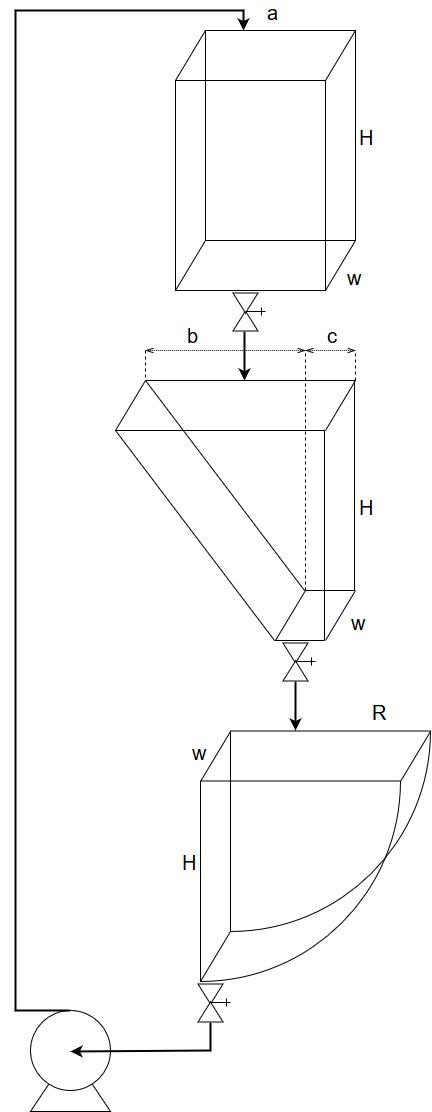
\includegraphics[scale=.5]{Grafika/schemat_zbiornikow}
	\caption{Układ zbiorników z zaznaczonymi wymiarami. Źródło: własne.}\label{fig:zbiorniki}
\end{figure}

\section{Wprowadzenie z zakresu dynamiki płynów}
\label{sec:plyny}

W niniejszym podrozdziale zostały przypomniane podstawowe prawa fizyki związane z przepływem cieczy oraz jego związkiem z poziomem tej cieczy w zbiorniku.

%-------------------------------------------------
\subsection{Równanie Bernoulliego i prawo Torricellego}
\label{sub:plyny-torr}

Równanie Bernoulliego jest jednym z podstawowych praw termodynamiki płynów idealnych. Mówi ono, że wzrost prędkości przepływu cieczy musi wiązać się ze spadkiem ciśnienia lub energii potencjalnej.
Ma kilka postaci; najpopularniejszą jest tzw. szczególne równanie Bernoulliego, które wiąże energię mechaniczną płynu z jego prędkością w danym miejscu, wysokością w układzie odniesienia służącym do wyznaczania energii potencjalnej, ciśnieniem i gęstością.
W takiej formie można je stosować tylko do cieczy nieściśliwych i nielepkich, jednocześnie zakładając stacjonarność i bezwirowość przepływu.

Ta szczególna postać równania Bernoulliego jest przedstawiona jako równanie \ref{eq:bernoulli}.

\begin{equation}\label{eq:bernoulli}
e_{m} = \frac{v^2}{2} + gh + \frac{p}{\rho} = const
\end{equation}

Oznaczenia:
\begin{itemize}
	\item $e_{m}$ - energia jednostki masy cieczy,
	\item $v$ - prędkość cieczy w danym miejscu,
	\item $g$ - przyspieszenie grawitacyjne,
	\item $h$ - wysokość w układzie odniesienia, w którym jest wyznaczana energia potencjalna,
	\item $p$ - ciśnienie cieczy w danym miejscu,
	\item $\rho$ - gęstość cieczy.
\end{itemize}

Z równania Bernoulliego można wyprowadzić bezpośrednią zależność między prędkością cieczy a jej poziomem w zbiorniku. Jest ona znana pod nazwą prawa Torricellego i przedstawiona jako równanie \ref{eq:torricelli} (przyjęto oznaczenia takie jak w przypadku równania \ref{eq:bernoulli}).
Można owo prawo zapisać w bardziej ogólnej formie słownej:

\begin{torricelli}
    Prędkość wypływu cieczy jest proporcjonalna do pierwiastka kwadratowego z poziomu cieczy w zbiorniku.
    \begin{equation}\label{eq:torricelli}
    v = \sqrt{2gh}
    \end{equation}
\end{torricelli}
Takie sformułowanie tego prawa będzie istotne w dalszych krokach wyznaczania modelu matematycznego rozważanego układu.


\subsection{Bilans masy}
\label{sub:plyny-bilans}

Kolejnym zjawiskiem fizycznym, którego zrozumienie jest potrzebne, aby wyznaczyć model matematyczny rozważanego w niniejszej pracy układu zbiorników, jest bilans masy, czyli bezpośrednia konsekwencja \emph{prawa zachowania masy}.

\begin{mass}
    Masa układu ciał (suma mas wszystkich ciał wchodzących w skład tego układu) nie zmienia się podczas przemian i oddziaływań fizycznych w nim zachodzących.
    \begin{equation}\label{eq:mass-conservation}
        m_{uk} = const
    \end{equation}
\end{mass}

Rozważając układ pojedynczego zbiornika z cieczą, do którego ta ciecz jest nalewana i z którego się ona wylewa, można sformułować następstwo tego prawa dane równaniem \ref{eq:mass-balance}. Mówi ono, że zmiana masy w rozważanym zbiorniku - $m_{zb}$ - jest równa zmianie masy do niego wpływającej - $m_{we}$ - i wypływającej - $m_{wy}$.

\begin{equation}\label{eq:mass-balance}
    \frac{\partial m_{we}}{\partial t} - \frac{\partial m_{wy}}{\partial t} =\frac{\partial m_{zb}}{\partial t}
\end{equation}

Przyjmując założenie, że ciecz w zbiorniku i poza nim ma stałą gęstość $\rho$ oraz stosując następujące podstawienia:
\begin{itemize}
    \item $m_{zb} = V_{zb}\cdot\rho$, gdzie $V_{zb}$ to objętość cieczy w zbiorniku,
    \item $V_{zb} = A_{zb} \cdot h_{zb}$, gdzie $A_{zb}$ to pole przekroju poprzecznego zbiornika, a $h_{zb}$ to wysokość słupa cieczy w tym zbiorniku
\end{itemize}
można przedstawić powyższą zależność w postaci opisanej zależnością \ref{eq:tank-mass-balance} (za: \cite{Postlethwaite}).

\begin{equation}\label{eq:tank-mass-balance}
    A_{zb} \cdot \frac{\partial h_{zb}}{\partial t} = \frac{\partial V_{we}}{\partial t} - \frac{\partial V_{wy}}{\partial t}
\end{equation}

Strumień (zmiana objętości cieczy w czasie) wypływający z takiego zbiornika można otrzymać na podstawie prawa Torricellego - jest on dany zależnością \ref{eq:tank-outflow}, gdzie $C$ to stała proporcjonalności wypływu. W rozważanym układzie będzie on zależeć od ustawienia zaworu wyjściowego z danego zbiornika, a więc można powiedzieć, że strumień opisuje opór wypływu ze zbiornika (za: \cite{TanksManual}).

\begin{equation}\label{eq:tank-outflow}
\frac{\partial V_{wy}}{\partial t} = C\cdot\sqrt{h_{zb}}
\end{equation}

Jeśli chodzi o strumień wpływający, to dla drugiego i trzeciego zbiornika jest on równy strumieniowi wypływającemu z poprzedniego zbiornika. Można przyjąć, że dla pierwszego zbiornika ten strumień to sterowanie pompą. Będzie ono oznaczone symbolem $u$.

Pola powierzchni przekrojów poprzecznych wszystkich trzech zbiorników przedstawiono jako równanie \ref{eq:model-fields}. Zastosowano oznaczenia z \ref{fig:zbiorniki}.

\begin{equation}\label{eq:model-fields}
    \begin{array}{lr}
        A_{1} = w \cdot a \\
        A_{2} = c\cdot w + \frac{h_{2}}{h_{max}}\cdot b\cdot w \\
        A_{3} = w\cdot \sqrt{R^{2} - (R - h_{3})^{2}}
    \end{array}
\end{equation}

%-------------------------------------------------
\subsection{Rodzaje przepływów}
\label{sub:plyny-przeplywy}

Przytoczona wcześniej szczególna postać równania Bernoulliego (równanie \ref{eq:bernoulli}) jest obwarowana założeniem stacjonarności przepływu. Oznacza to dwie rzeczy:
\begin{enumerate}
    \item Wartości wektorów prędkości cieczy są stałe w czasie.
    \item Poszczególne ,,warstwy'' cieczy nie wpływają na siebie.
\end{enumerate}

Drugi z tych warunków jest znany pod nazwą przepływu laminarnego, który zwykle ma miejsce przy niskich prędkościach cieczy. W takim typie przepływu nie występują żadne jego zaburzenia (ruchy wirowe, prądy przeciwne itp.), a zachowanie poszczególnych ,,warstw'' cieczy porównać można do tasowania kart: przepływają obok siebie bez wpływania jedna na drugą. Jej cząstki będące blisko powierzchni przemieszczają się po liniach równoległych do tafli cieczy.

Niestety, w rzeczywistości ciężko jest spełnić założenie laminarności przepływu, nie mówiąc już o jego stacjonarności. W związku z tym można zastosować pewne praktyczne uogólnienie zależności \ref{eq:tank-outflow} w stosunku do cieczy wypływających w sposób nielaminarny. Polega ono na zastąpieniu pierwiastka we wspomnianym wzorze parametrem $\alpha$, którego wartość można dobrać na podstawie pomiarów w rzeczywistym układzie (przykład podany w \cite{TanksManual}). Uwzględniają to uogólnienie, można zapisać nowe sformułowanie zależności \ref{eq:tank-outflow} jako równanie \ref{eq:tank-outflow-nonlmnr}.

\begin{equation}\label{eq:tank-outflow-nonlmnr}
    \frac{\partial V_{wy}}{\partial t} = C\cdot h_{zb}^{\alpha}
\end{equation}


\section{Model matematyczny zestawu zbiorników}
\label{sec:model}

Na podstawie podanych wcześniej zależności można zdefiniować model matematyczny rozważanego układu zbiorników.
Jest on dany równaniem \ref{eq:model} (za: \cite{TanksManual}).

\begin{equation}\label{eq:model}
\left \{
\begin{array}{lr}
\frac{\partial h_{1}}{\partial t} = \frac{u - C_{1}{h_{1}}^{\alpha_{1}}}{aw} \\[8pt]
\frac{\partial h_{2}}{\partial t} = \frac{C_{1}{h_{1}}^{\alpha_{1}} -  C_{2}{h_{2}}^{\alpha_{2}}}{cw + \frac{h_{2}}{h_{max}}bw} \\[12pt]
\frac{\partial h_{3}}{\partial t} = \frac{C_{2}{h_{2}}^{\alpha_{2}} -  C_{3}{h_{3}}^{\alpha_{3}}}{w\sqrt{R^{2} - (R - h_{3})^{2}}}
\end{array}
\right.
\end{equation}

Oznaczenia:
\begin{itemize}
    \item $h(t) = [h_{1}(t)~ h_{2}(t)~ h_{3}(t)]^{T}$ - poziomy wody w zbiornikach,
    \item $u(t)$ - sterowanie pompą,
    \item $a$ - szerokość pierwszego zbiornika,
    \item $b$ - szerokość trójkątnej części drugiego zbiornika,
    \item $c$ - szerokość prostopadłościennej części drugiego zbiornika,
    \item $R$ - promień trzeciego zbiornika,
    \item $w$ - głębokość zbiorników,
    \item $h_{max}$ maksymalna wysokość słupa wody w zbiornikach,
    \item $C_{i}$ - opór wypływu z $i$-tego zbiornika,
    \item $\alpha_{i}$ - współczynnik wypływu z $i$-tego zbiornika.
\end{itemize}

Wszystkie wymiary w powyższym wzorze zostały przedstawione na rys. \ref{fig:zbiorniki}. Są na nim również oznaczone opory wypływów $C_{1}$ - $C_{3}$ przy odpowiednich zaworach.

Przyjmując $\alpha_{i} = \frac{1}{2}, \forall_{i \in \{1, 2, 3\}}$, można uszczegółowić powyższy model, zakładając tylko przepływ laminarny.
Taka właśnie jego postać będzie wykorzystywana przy analitycznym wyznaczeniu współczynników równania sprzężonego (definicja znajduje się w sekcji \ref{sub:toc-def-intro}), które jest przeprowadzone w podrozdziale \ref{sub:toc-ctrl}.
W rzeczywistości, jak zostało wspomniane w podrozdziale \ref{sub:plyny-przeplywy}, wartości tych współczynników będą musiały być trochę mniejsze, aby oddać faktyczny sposób przepływu wody między zbiornikami.

W rozważanym układzie zbiorników przyjmuje się następujące ograniczenia (pomijając oczywiste $t \geq 0$):
\begin{itemize}
    \item ograniczenia równościowe:
    \begin{equation}\label{eq:model-eq-const}
    \begin{array}{lr}
        h_{1}(0) = h_{10}\\
        h_{2}(0) = h_{20}\\
        h_{3}(0) = h_{30}\\
    \end{array}
    \end{equation}
    \item ograniczenia nierównościowe:
    \begin{equation}\label{eq:model-noneq-const}
    \begin{array}{lr}
        \forall_{t \in [0, T]}:~ 0 \leq h_{1}(t) \leq h_{max}\\
        \forall_{t \in [0, T]}:~ 0 \leq h_{2}(t) \leq h_{max}\\
        \forall_{t \in [0, T]}:~ 0 \leq h_{3}(t) \leq h_{max}\\
        \forall_{t \in [0, T]}:~ 0 \leq u(t) \leq u_{max}
    \end{array}
    \end{equation}
\end{itemize}
Parametry $h_{10}$, $h_{20}$ i $h_{30}$ oraz $h_{max}$ traktuje się jako zadane.

Punkty równowagi (nazywane również stanami ustalonymi) takiego systemu będą opisane przez zależność \ref{eq:steady-state-def-model} i wyznaczone przez parę wektora wartości zmiennych stanu $h_{r}$ oraz sterowania $u_{r}$. Brak zależności od czasu owej pary został odpowiednio odnotowany.

\begin{equation}\label{eq:steady-state-def-model}
\frac{\partial h(t)}{\partial t} = 0 ~\Rightarrow~ 
\left \{
\begin{array}{lr}
    \frac{\partial h_{1}}{\partial t} = 0 \\
    \frac{\partial h_{2}}{\partial t} = 0 \\
    \frac{\partial h_{3}}{\partial t} = 0
\end{array}
\right.
\end{equation}

Dla rozważanego układu zbiorników będą miały postać daną zależnością \ref{eq:model-steady-state}.

\begin{equation}\label{eq:model-steady-state}
\begin{array}{lr}
u_{r} = C_{1}h_{1}^{\alpha_{1}} = C_{2}h_{2}^{\alpha_{2}} = C_{3}h_{3}^{\alpha_{3}}\\
h_{r} = \begin{bmatrix}
h_{1r}\\h_{2r}\\h_{3r}
\end{bmatrix}
=
\begin{bmatrix}
\big( \frac{\textstyle u_{r}}{\textstyle C_{1}}\big)^{\frac{\scriptstyle 1}{\scriptstyle \alpha_{1}}}\\
\big( \frac{\textstyle u_{r}}{\textstyle C_{2}}\big)^{\frac{\scriptstyle 1}{\scriptstyle \alpha_{2}}}\\
\big( \frac{\textstyle u_{r}}{\textstyle C_{3}}\big)^{\frac{\scriptstyle 1}{\scriptstyle \alpha_{3}}}
\end{bmatrix}
\end{array}
\end{equation}

Wynika z tego, że układ otwarty jest asymptotycznie stabilny, gdyż posiada tylko jeden, zerowy punkt równowagi (pokazany jako wzór \ref{eq:model-zero-state}). Jest to również zgodne z fizyczną naturą tego systemu zbiorników: przy braku zasilania go pompą, cała woda wycieknie ze wszystkich trzech zbiorników.

\begin{equation}\label{eq:model-zero-state}
h_{r}^{0} = \begin{bmatrix}
h_{1r}^{0}\\h_{2r}^{0}\\h_{3r}^{0}
\end{bmatrix} = 
\begin{bmatrix}
0\\0\\0
\end{bmatrix}
\end{equation}


\chapter{Regulacja optymalna}
\label{cha:reg-opt}

W niniejszym rozdziale zostały opisane matematyczne podstawy wyznaczania sterowania optymalnego według dwóch wskaźników jakości występujących w niniejszej pracy:
\begin{itemize}
    \item czas (regulacja czasooptymalna),
    \item liniowo-kwadratowego (regulacja liniowo-kwadratowa).
\end{itemize}


\section{Regulacja czasooptymalna}
\label{sec:toc}

W niniejszym podrozdziale przedstawiona została koncepcja regulacji czasooptymalnej. Zostały podane założenia zagadnienia, twierdzenia, na których podstawie można wyliczyć rozwiązanie oraz jego proponowana forma analityczna.

Zaznacza się, że mimo iż podane niżej definicje i założenia są wzięte z ogólnych zagadnień optymalizacji dynamicznej, to w podanym brzmieniu stosują się tylko do zagadnienia wyznaczania sterowania czasooptymalnego.

%-------------------------------------------------
\subsection{Ogólna definicja zagadnienia}
\label{sub:toc-def}

%-------------------
\subsubsection{Założenia wstępne}
\label{sub:toc-def-intro}
Dany jest układ opisany stacjonarnym, zwyczajnym równaniem różniczkowym (pokazanym jako równanie \ref{eq:general_system}), w którym:

\begin{equation}\label{eq:general_system}
    \frac{\partial x(t)}{\partial t} = f(x(t), u(t)), ~ 0 \leq t \leq T
\end{equation}

\begin{itemize}
    \item wektor zmiennych stanu w chwili $t$ - $x(t)$ spełnia następujące założenia:
    \begin{itemize}
        \item $\forall_{t \geq 0}:~ x(t) \in \mathbb{R}^{n}$ - ma $n$ składowych, a więc rozważany system ma $n$ równań różniczkowych zwyczajnych,
        \item $x(0) = x_{0} \in \mathbb{R}^{n}$ - spełnia warunek początkowy $x_{0}$;
    \end{itemize}
    \item wektor sterowań w chwili $t$ - $u(t)$:
    \begin{itemize}
        \item $\forall_{t \geq 0}:~ u(t) \in D \subset \mathbb{R}^{m}$ - ma $m$ składowych zawierającym się w zbiorze $D$ ograniczającym wartości sterowań,
        \item $u(0) = u_{0}$ - spełnia warunek początkowy $u_{0}$,
        \item funkcja $u$ jest przedziałami ciągła na przedziale $[0, T]$ (dokładny opis w \cite{Korytowski2015}), czyli:
        \begin{itemize}
            \item ma co najwyżej skończoną liczbę punktów nieciągłości,
            \item w każdym z nich ma skończoną granicę lewostronną,
            \item jest prawostronnie ciągła,
            \item w lewym końcu przedziału jest lewostronnie ciągła;
        \end{itemize}
    \end{itemize}
    \item funkcja $f: \mathbb{R}^{n} \times \mathbb{R}^{m} \longmapsto \mathbb{R}^{n}$:
    \begin{itemize}
        \item $f \in C^{1}$ - jest ciągła i różniczkowalna ze względu na pierwszy argument,
        \item $\frac{\partial f(t)}{\partial x} \in C^{0}$ - jej pochodna ze względu na pierwszy argument jest ciągła.
    \end{itemize}
\end{itemize}

Rozwiązaniem takiego równania jest oczywiście funkcja $x: [0, T) \longmapsto \mathbb{R}^{n}$ nazywana \emph{trajektorią układu}. 

Trajektoria będąca rozwiązaniem zagadnienia minimalnoczasowego musi spełniać następujący warunek końcowy (nazywany również stanem docelowym):
\begin{equation}\label{eq:final_term}
    x(T) = x_{f} \in \mathbb{R}^{n}
\end{equation}

Ów czas $T$, po którym przy danym sterowaniu stan systemu osiągnie warunek końcowy, będzie wskaźnikiem jakości: 
\begin{equation}\label{eq:quality}
    Q(u(t)) = q(x_{f}) = T
\end{equation}

Na tej podstawie można określić \emph{sterowanie optymalne} $\hat{u}(t)$, które spełnia wszystkie wspominane przy opisie równania \ref{eq:general_system} warunki oraz zależność \ref{eq:optimal_quality}. Trajektoria układu wygenerowana przez zastosowanie sterowania optymalnego nazwana jest \emph{trajektorią optymalną} i opisana symbolem $\hat{x}(t)$.
\begin{equation}\label{eq:optimal_quality}
    \forall_{u(t)}:~ Q(u(t)) \leq Q(\hat{u}(t))
\end{equation}

W opisie zagadnienia czasooptymalnego potrzebne są jeszcze dwa pojęcia.
Pierwsze to \emph{funkcja sprzężona} $\psi: [0, T] \longmapsto \mathbb{R}^{n}$ będąca rozwiązaniem tzw. równania sprzężonego \ref{eq:costate-def}.
\begin{equation}\label{eq:costate-def}
\frac{\partial \psi(t)}{\partial t} = - \frac{\partial f(x(t), u(t)}{\partial x}
\end{equation}

Tak, jak w przypadku trajektorii optymalnej układu, trajektoria $\psi(t)$ wyznaczona w układzie, w którym zastosowane zostało sterowanie optymalne $\hat{u}(t)$, nosi nazwę \emph{trajektorii sprzężonej optymalnej} i oznaczona jest symbolem $\hat{\psi}(t)$.

Ostatnim pojęciem potrzebnym w niniejszym zagadnieniu jest \emph{hamiltonian}, zwany również \emph{funkcją Hamiltona}, czyli funkcja $H: \mathbb{R}^{n} \times \mathbb{R}^{n} \times \mathbb{R}^{m} \longmapsto \mathbb{R}$ który dla trajektorii układu $x(t)$ wygenerowanej przy pomocy sterowania $u(t)$ i odpowiadającej im trajektorii sprzężonej $\psi(t)$ zdefiniowany jest zależnością \ref{eq:hamiltonian-def}.

\begin{equation}\label{eq:hamiltonian-def}
H(\psi(t), x(t), u(t)) = \psi(t) \circ f(x(t), u(t)) = \psi(t)^{T} \cdot f(x(t), u(t))
\end{equation}

%-------------------
\subsubsection{Zasada maksimum Pontriagina}
\label{sub:toc-def-pontriagin}

Aby jednoznacznie opisać, a następnie wyznaczyć sterowanie czasooptymalne, potrzebne jest przytoczenie zasadniczego twierdzenia w optymalizacji dynamicznej. Jest ono znane pod nazwą \emph{zasada maksimum Pontriagina}. Zostało opracowane w 1956 r. przez rosyjskiego matematyka Lwa Pontriagina. Twierdzenie podaje się w brzmieniu z \cite{Korytowski2015}.

\begin{pontriagin-max}\label{the:pontryagin}
    Zakładając układ opisany równaniem \ref{eq:general_system} z warunkiem końcowym \ref{eq:final_term} i wskaźnikiem jakości \ref{eq:quality} oraz równanie sprzężone \ref{eq:costate-def}:
    jeśli dla trajektorii układu $\hat{x}(t)$ wygenerowanej przy pomocy sterowania $\hat{u}(t)$ i odpowiadającej im trajektorii sprzężonej $\hat{\psi}(t)$ zachodzi:
    \begin{equation}\label{eq:pontriagin}
    \forall_{u(t) \in D}~ \forall_{t \in [0, T]}:~ H(\hat{\psi}(t), \hat{x}(t), \hat{u}(t)) ~ \geq ~ H(\hat{\psi}(t), \hat{x}(t), u(t))
    \end{equation}
    to sterowanie $\hat{u}(t)$ jest sterowaniem optymalnym.
\end{pontriagin-max}

Dowód zasady maksimum nie został uwzględniony w tej pracy. Można go znaleźć w \cite{Korytowski2015} oraz w \cite{Evans}.

Powyższe twierdzenie należy obwarować dodatkowymi warunkami koniecznymi optymalności. Niech funkcja $g: \mathbb{R}^{2n} \longmapsto \mathbb{R}^{l}$ opisuje zestaw ograniczeń nierównościowych, a funkcja $h: \mathbb{R}^{2n} \longmapsto \mathbb{R}^{k}$ - ograniczeń równościowych. Obie dane są wzorem \ref{eq:pontryagin-constraints}. Dodatkowo zakłada się, że $g, h \in C^{1}$.
\begin{equation}\label{eq:pontryagin-constraints}
    \begin{array}{lr}
    g(x_{0}, x_{f}) \leq 0 \\
    h(x_{0}, x_{f}) = 0
    \end{array}
\end{equation}

Ponadto, zakłada się, że istnieją $\lambda \in \mathbb{R}$, $\mu \in \mathbb{R}^{l}$ oraz $\rho \in \mathbb{R}^{k}$, które wraz z uprzednio zdefiniowanymi wielkościami i funkcjami spełniają następujące \emph{warunki konieczne optymalności}:
\begin{itemize}
    \item warunek nieujemności:
    \begin{equation}\label{eq:pontryagin-noneg}
    \lambda \geq 0 \land \|\mu\| \geq 0
    \end{equation}
    \item warunek nietrywialności:
    \begin{equation}\label{eq:pontryagin-notriv}
    \lambda + \|\mu\| + \|\rho\| > 0
    \end{equation}
    \item warunek komplementarności:
    \begin{equation}\label{eq:pontryagin-comp}
    \mu \circ g(x_{0}, x_{f}) = 0
    \end{equation}
    \item warunki transwersalności:
    \begin{equation}\label{eq:pontryagin-trans}
    \begin{array}{lr}
        \hat{\psi}(0) = \frac{\partial (\mu \circ g + \rho \circ h)}{\partial x_{0}}\\[8pt]
        \hat{\psi}(T) = - \frac{\partial (\mu \circ g + \rho \circ h)}{\partial x_{f}}\\[8pt]
        \forall_{t \in [0, T]}:~ H(\psi(t), x(t), u(t)) = \frac{\partial (\lambda T + \mu \circ g + \rho \circ h)}{\partial T} = \lambda
    \end{array}
    \end{equation}
    \item równanie sprzężone dane wzorem \ref{eq:costate-def},
    \item warunek maksimum hamiltonianu dany nierównością \ref{eq:pontriagin}.
\end{itemize}


%-------------------------------------------------
\subsection{Nieliniowość układu a sterowanie czasooptymalne}
\label{sub:toc-nonlnr}

Poszukiwanie sterowania czasooptymalnego w systemach nieliniowych jest w ogólności bardzo skomplikowane, przede wszystkim ze względu na trudność rozwiązania analitycznego nieliniowych (lub nawet niestacjonarnych) równań różniczkowych. Układ zbiorników omawiany w niniejszej pracy również takie posiada: zarówno równania dynamiki układu \ref{eq:model}, jak i równania sprzężone \ref{eq:model-costate} są nieliniowe.

Aby uprościć analizę problemu oraz fizyczne zastosowanie wyznaczonego sterowania, zakłada się, że poszukiwane jego postaci będą klasy ,,bang - bang''. To znaczy, że będą przyjmowały tylko wartości z brzegów jednowymiarowego zbioru dopuszczalnego $D \in \mathbb{R} \land D = [0, u_{max}] \Rightarrow \forall_{t \in [0, T]}:~ u(t) \in [0, u_{max}]$.

\begin{equation}\label{eq:nonlin-bang-bang}
    \frac{\partial x}{\partial t} = f(x(t)) + \sum_{i=1}^{m} g_{i}(x(t)) \cdot u_{i}(t)
\end{equation}

Można przyjąć takie założenie, ze względu na to, iż (jak pokazano w \cite{YiMa2008} oraz w rozdziale 7.10 \cite{AthansOptCtrl}) dla systemów, których równania mają postać opisaną równaniem \ref{eq:nonlin-bang-bang} (a taką dokładnie ma omawiany układ z $m = 1$), funkcja przełączająca ma wtedy postać: $\phi(t) = \hat{\psi}(t) \circ g(\hat{x}(t))$. Owa funkcja opisuje momenty, w których sterowanie zmienia swoją wartość z jednego krańca zbioru $D$ na drugi. W przypadku rozważanego układu zbiorników sterowanie optymalne będzie dane wzorem \ref{eq:model-opt-ctrl}.

\begin{equation}\label{eq:model-opt-ctrl}
\begin{array}{lr}
    \hat{u}(t) = \frac{sgn(\phi(t)) + sgn(\phi(t))^{2}}{2} \cdot u_{max} ~ \land ~ \phi(t) = \frac{\hat{\psi}_{1}(t)}{aw} \Rightarrow \\
    \hat{u}(t) = \frac{sgn(\hat{\psi}_{1}(t) + sgn(\hat{\psi}_{1}(t))^{2}}{2} \cdot u_{max}
\end{array}
\end{equation}

Dodatkowo, jak wspomniano w podrozdziale \ref{sec:model}, układ otwarty jest stabilny, a ograniczone sterowanie nie może tego zmienić.

Podobne założenia są częstą praktyką w analizie stabilnych systemów nieliniowych ze względu na prostotę fizycznej aplikacji sterowania ,,bang - bang''. Przykłady znajdują się m.in. w \cite{VakKek82}, \cite{BalSom83} oraz \cite{Itik2016}.

%-------------------------------------------------
\subsection{Analityczne metody wyznaczania sterowania czasooptymalnego}
\label{sub:toc-ctrl}

Analityczne rozwiązania poszukiwania sterowania czasooptymalnego zwykle opierają się bezpośrednio na przytoczonej powyżej zasadzie maksimum i warunkach koniecznych optymalności. W niniejszym podrozdziale zostanie pokrótce przedstawiona droga mogąca zmierzać do wyznaczenia analitycznego czasooptymalnego sterowania w rozważanym układzie zbiorników. Całe rozwiązanie nie jest przeprowadzone ze względu na fakt, iż równania sprzężone są niestacjonarne, a więc ich rozwiązanie analityczne byłoby bardzo trudne lub wręcz niemożliwe.

Pierwszym krokiem ku wyliczeniu analitycznego rozwiązania jest wyznaczenie równań sprzężonych za pomocą wzoru \ref{eq:costate-def}. Przyjmując współczynniki $\alpha_{i} = \frac{1}{2} \forall_{i \in \{1, 2, 3\}}$ w modelu matematycznym zestawu zbiorników danym równaniem \ref{eq:model}, można wyznaczyć równania sprzężone rozważanego układu. Są one dane wzorem \ref{eq:model-costate}. Pominięto w nim zależności wszystkich funkcji $\psi$ oraz $h$ od czasu, aby uprościć zapis.

\begin{equation}\label{eq:model-costate}
	\left \{
	\begin{array}{lr}
		\frac{\partial \psi_{1}}{\partial t} =  \psi_{1}\frac{C_{1}}{2aw\sqrt{h_{1}}} - \psi_{2}\frac{C_{1}}{2\sqrt{h_{1}}(cw + \frac{h_{2}}{h_{max}}bw)} \\[20pt]
		\frac{\partial \psi_{2}}{\partial t} = - \psi_{2}\frac{1}{cw + \frac{h_{2}}{h_{max}}bw}(\frac{b(C_{1}\sqrt{h_{1}} - C_{2}\sqrt{h_{2}})}{ch_{max} + bh_{2}} - \frac{C_{2}}{2\sqrt{h_{2}}}) - \psi_{3}\frac{1}{w\sqrt{h_{3}(2R - h_{3})}} \\[20pt]
		\frac{\partial \psi_{3}}{\partial t} = \psi_{3}\frac{-C_{3}(3R - 2h_{3})}{wh_{3}(2R - h_{3})^{\frac{3}{2}}}
	\end{array}
	\right.
\end{equation}

Następnie trzeba by przedefiniować ograniczenia równościowe (dane wzorem \ref{eq:model-eq-const}) i nierównościowe (\ref{eq:model-noneq-const}) tak, aby spełniały założenia funkcji $g$ i $h$ opisane zależnościami \ref{eq:pontryagin-constraints}.
Dodatkowo należy dopisać od ograniczeń równościowych to wynikające z faktu poszukiwania sterowania czasooptymalnego, czyli \ref{eq:final_term}, które w tym przypadku będzie miało postać opisaną przez \ref{eq:model-final-term}, gdzie $h_{1f}$, $h_{2f}$ i $h_{3f}$ są dane.

\begin{equation}\label{eq:model-final-term}
\begin{array}{lr}
    h_{1}(T) = h_{1f}\\
    h_{2}(T) = h_{2f}\\
    h_{3}(T) = h_{3f}
\end{array}
\end{equation}

Korzystając z warunków komplementarności (\ref{eq:pontryagin-comp}) oraz nieujemności (\ref{eq:pontryagin-noneg}), powinno się wyznaczyć składowe wektora $\mu$ oraz założyć pewną postać wektora $\rho$ (bazując takie założenie na \ref{eq:pontryagin-notriv}).

Na podstawie tych danych należałoby wyznaczyć warunki początkowy i końcowy danym wzorem \ref{eq:pontryagin-trans} dla powyższych równań sprzężonych, co pozwoliłoby wyznaczyć analityczne wzory opisujące wszystkie składowe trajektorii sprzężonych systemu.

Na koniec, korzystając z zależności \ref{eq:model-opt-ctrl}, można by wyznaczyć analityczny wzór sterowania optymalnego.


%-------------------------------------------------
\subsection{Numeryczne metody wyznaczania sterowania czasooptymalnego}
\label{sub:toc-num}

W niniejszej sekcji zostały przekrojowo zaprezentowane numeryczne metody poszukiwania sterowania czasooptymalnego dla układów nieliniowych.
Nie jest jej celem przedstawiać dokładne działanie wszystkich istniejących algorytmów, ale raczej dokonać klasyfikacji i naświetlić interesujące metody oraz odesłać do odpowiedniej literatury przedmiotu.

Ogólna definicja problemu optymalizacji rozwiązywanego przez takie metody została dana w sekcji \ref{sub:toc-def}, tutaj należy ją uzupełnić o ogólną postać funkcjonału $Q$ będącego wskaźnikiem jakości w rozpatrywanym zadaniu. Jest ona dana równaniem \ref{eq:num-oc-quality} (za: \cite{Rao2010}) i składa się z:
\begin{itemize}
    \item wyrażenia podcałkowego $L$ zależącego od:
    \begin{itemize}
        \item czasu,
        \item stanu $x(t)$,
        \item sterowania $u(t)$,
        \item parametrów statycznych układu $p$,
        \item czasu końcowego $T$;
    \end{itemize}
    \item wyrażenia $M$ zależącego od:
    \begin{itemize}
        \item czasu początkowego optymalizacji $t_{0}$,
        \item stanu początkowego $x(t_{0})$,
        \item stanu końcowego $x(T)$,
        \item parametrów statycznych układu $p$,
        \item czasu końcowego $T$.
    \end{itemize}
\end{itemize}

\begin{equation}\label{eq:num-oc-quality}
Q[x(\cdot), u(\cdot), p, T] = \int_{t_{0}}^{T}L(\tau, x(\tau), u(\tau), p, T)d\tau + M(t_{0}, x(t_{0}), x(T), p, T)
\end{equation}

Gdy we wskaźniku jakości występuje tylko człon podcałkowy, to mówi się, że jest postaci Lagrange'a. Jeśli ma tylko drugi człon, nazywa się go postacią Mayera. Sytuację, w której występują oba, określa się mianem postaci Boltza. Oczywiście, podział między członami jest umowny i można ten sam funkcjonał zapisać zarówno w postaci Lagrange'a, jak i Mayera. Przykładem jest rozpatrywany w niniejszej pracy wskaźnik jakości dany postacią Mayera we wzorze \ref{eq:quality}. Równie dobrze można by go zapisać w postaci Lagrange'a: $Q = \int_{0}^{T} 1 ~d\tau$.

Podstawowy podział metod obliczeniowych to metody \emph{pośrednie} oraz \emph{bezpośrednie}, choć ich rozróżnienie nie jest ścisłe i istnieją metody łączące cechy obu tych klas (za: \cite{Betts98}).

Pierwsze z nich polegają na dyskretyzacji sterowania (czasem również stanu), aby móc przybliżyć wyjściowy problem optymalizacji dynamicznej zadaniem optymalizacji statycznej: programowania nieliniowego (ang. \emph{NLP - Non-Linear Programming})lub optymalizacji nieliniowej. To przybliżenie jest zwykle aproksymacją sterowań (oraz stanów w tych metodach, które z nich korzystają) w konkretnych przedziałach czasu wielomianami. Dzięki temu zastępuje się nieskończenie wymiarowy problem optymalizacji takim o skończonym wymiarze. Ta klasa metod jest bardziej uniwersalna i mniej wrażliwa na błędy, ale stosunkowo wolniej zbieżna i przez to mniej dokładna (za: \cite{Korytowski2015}). Przykładowe metody bezpośrednie przedstawione są poniżej:
\begin{itemize}
    \item optymalizacja czasów przełączeń (do zastosowania tylko w przypadku sterowania o postaci ,,bang-bang''),
    \item parametryzacja sterowania (np. aproksymacja funkcją schodkową),
    \item bezpośrednie metody kolokacyjne,
    \item metody strzałów bezpośrednich.
\end{itemize}

Drugie wykorzystują warunki konieczne optymalności oryginalnego zadania i sprowadzają je do problemu granicznego lub dwugranicznego, który jest dany układem równań bazującym na zasadzie maksimum Pontriagina. Rozwiązanie takiego układu równań skutkuje wyznaczeniem trajektorii układu będących potencjalnie rozwiązaniem problemu. Każdą z nich bada się, jakeigo rodzaju ekstremem jest: minimum, maksimum lub punktem siodłowym, a następnie wybiera się taką, której koszt jest najmniejszy. Metody pośrednie wymagają dobrze dobranej trajektorii początkowej układu, która zawiera informacje na temat struktury sterowania (za: \cite{Korytowski2015}). W niniejszej pracy zostało to również zaobserwowane i opisane w sekcji \ref{sub:opt-init}. Jest to wada tego rodzaju metod - wymagają większego nakładu pracy analitycznej przed rozpoczęciem obliczeń, aby wyznaczyć odpowiedni punkt startowy dla algorytmu. Zaletą za to jest dużo szybsza zbieżność w otoczeniu rozwiązania (za: \cite{Korytowski2015}). Przykładowe metody pośrednie to:
\begin{itemize}
    \item pośrednia metoda strzałów,
    \item pośrednia metoda strzałów wielokrotnych,
    \item pośrednie metody kolokacyjne.
\end{itemize}

Rys. \ref{fig:num-methods} przedstawia operacje matematyczne wykorzystywane przez oba rodzaje metod rozwiązywania problemów optymalizacji dynamicznej. Dokładniejszy opis metod wykonujących te operacje znajduje się w \cite{Rao2010}.

\begin{figure}[htp]
    \centering
    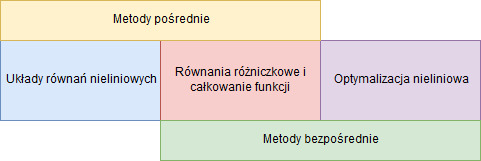
\includegraphics[scale=0.8]{Grafika/num-methods}
    \caption{Trzy główne komponenty wyznaczania sterowania optymalnego i klasy metod, które z nich korzystają. Źródło: \cite{Rao2010}. Tłumaczenie: własne.}
    \label{fig:num-methods}
\end{figure}


\section{Regulacja liniowo - kwadratowa}
\label{sec:lqr}

W niniejszym podrozdziale zostanie przedstawione zagadnienie szukania sterowania w układach liniowych z tzw. liniowo-kwadratowym wskaźnikiem jakości oraz nieskończonym horyzontem czasowym. Pokazana zostanie również metoda zastosowania takiego typu regulacji dla układów nieliniowych przy użyciu linearyzacji w punkcie pracy. Zostanie również pokrótce omówione zagadnienie doboru wag w wyznaczaniu regulatora liniowo-kwadratowego.

%-------------------------------------------------
\subsection{Ogólna definicja zagadnienia}
\label{sub:lqr-def}

Dany jest układ opisany liniowym równaniem różniczkowym \ref{eq:lqr-system} z wektorem zmiennych stanu $x(t) \in \mathbb{R}^{n}$ i warunkiem początkowym dla nich $x(0) = x_{0}$. Sterowaniem w tym układzie jest $u(t) \in \mathbb{R}^{m}$. Jak zostało wspomniane wyżej, horyzont czasowy jest nieskończony. Cały układ jest analogiczny do opisanego w sekcji \ref{sub:toc-def}.

\begin{equation}\label{eq:lqr-system}
\frac{\partial x(t)}{\partial t} = Ax(t) + Bu(t),~ 0 \leq t < \infty
\end{equation}

Przyjmuje się również wskaźnik jakości w tym układzie dany wzorem \ref{eq:lqr-quality}.
\begin{equation}\label{eq:lqr-quality}
Q(u(t)) = \frac{1}{2}\int_{0}^{\infty} \Big(x(t)^{T}Wx(t) + u(t)^{T}Ru(t)\Big)dt
\end{equation}

Dodatkowo zakłada się następujące właściwości macierzy wymienionych w powyższym wzorze:
\begin{itemize}
    \item macierz $W = W^{T} \geq 0$ - jest symetryczna i nieujemnie określona,
    \item macierz $R = R^{T} > 0$ - jest symetryczna i dodatnio określona (jest również czasem w literaturze oznaczana symbolem $Q$, gdy wskaźnik jakości jest oznaczony symbolem $J$).
\end{itemize}

Oczywiście, aby istniało sterowanie optymalne, musi istnieć również całka będąca wskaźnikiem jakości - jest to warunek konieczny i wystarczający. Sterowalność pary $A$ i $B$ lub asymptotyczna stabilność macierzy $A$ jest warunkiem wystarczającym. Oba są podane w \cite{Korytowski2015} oraz w \cite{AthansOptCtrl}.

Wyznaczenie sterowania optymalnego w tak zdefiniowanym problemie opiera się na rozwiązaniu algebraicznego równania Ricattiego (danego zależnością \ref{eq:ricatti-algebraic}) przy założeniu, że macierz $K$ jest symetryczna i nieujemnie określona. Jest ono opisane szerzej w \cite{AthansOptCtrl}, \cite{Korytowski2015} i \cite{Murray2006}.

\begin{equation}\label{eq:ricatti-algebraic}
KBR^{-1}B^{T}K - A^{T}K - KA - W =0
\end{equation}

Sterowanie optymalne $\hat{u}(t)$ ma wówczas postać daną wzorem \ref{eq:lqr-opt-ctrl}.
\begin{equation}\label{eq:lqr-opt-ctrl}
\hat{u}(t) = -R^{-1}B^{T}Kx(t),~ t \geq 0
\end{equation}

Aby taki regulator zapewnił asymptotyczną stabilność kontrolowanego układu, para $(W, A)$ musi być wykrywawlna, a para $(A, B)$ - stabilizowalna (za: \cite{Korytowski2015}).

%-------------------------------------------------
\subsection{Linearyzacja modelu}
\label{sub:lqr-lin}

Mimo iż podstawowa definicja zagadnienia liniowo kwadratowego zakłada liniowość sterowanego układu (jak we wzorze \ref{eq:lqr-system}), to można rozszerzyć jego zastosowanie również na układy nieliniowe przez użycie linearyzacji w otoczeniu punktu pracy.

Niech będzie dany układ opisany przez \ref{eq:general_system} wraz ze wszystkimi założeniami opisanymi w sekcji \ref{sub:toc-def-intro}.
Można go stabilizować tylko w jednym z jego punktów równowagi $(x_{r}, u_{r})$ (definiowanych równaniem \ref{eq:steady-state-points}) ze względu na to, iż tylko do takich punktów układ może dążyć w nieskończoności, która jest horyzontem czasowym analizowanego zagadnienia.

\begin{equation}\label{eq:steady-state-points}
\frac{\partial x(t)}{\partial t} = 0 ~\Rightarrow~ f(x_{r}(t), u_{r}(t)) = 0
\end{equation}

Na podstawie takiego punktu równowagi definiuje się odchyłki od stanu i sterowania ustalonego dane zależnością \ref{eq:lqr-deltas}.

\begin{equation}\label{eq:lqr-deltas}
\begin{array}{lr}
    \Delta x(t) = x(t) - x_{r}\\
    \Delta u(t) = x(t) - u_{r}
\end{array}
\end{equation}

Przy użyciu tak zdefiniowanych odchyłek wyjściowy nieliniowy układ można aproksymować układem liniowym (dany wzorem \ref{eq:lqr-nonlnr-system}) w pewnym otoczeniu owych odchyłek.

\begin{equation}\label{eq:lqr-nonlnr-system}
\begin{array}{lr}
    \frac{\partial \Delta x(t)}{\partial t} = \bar{A}\Delta x(t) + \bar{B}\Delta u(t)
\end{array}
\end{equation}

Macierze $A$ i $B$ zostały uzyskane w procesie linearyzacji funkcji $f(x(t), u(t))$ w punkcie $(x_{r}, u_{r})$ - wzór \ref{eq:lqr-nonlnr-matrices} pokazuje sposób, w jaki są zdefiniowane.

\begin{equation}\label{eq:lqr-nonlnr-matrices}
\begin{array}{lr}
    \bar{A} = \bigg(\left. \frac{\partial f(x(t), u_{r})}{\partial x(t)}\right\vert_{x(t) = x_{r}}\bigg)^{T}\\
    \bar{B} = \bigg(\left. \frac{\partial f(x_{r}, u(t))}{\partial u(t)}\right\vert_{u(t) = u_{r}}\bigg)^{T}
\end{array}
\end{equation}

Wskaźnik jakości dla takiego systemu również przyjmuje postać odchyłkową zaprezentowaną jako równanie \ref{eq:lqr-nonlnr-quality}. Założenia co do macierzy $W$ i $R$ są dalej takie same.

\begin{equation}\label{eq:lqr-nonlnr-quality}
Q(\Delta u(t)) = \frac{1}{2}\int_{0}^{\infty} \Big( \Delta x(t)^{T}W\Delta x(t) + \Delta u(t)^{T}R\Delta u(t) \Big)dt
\end{equation}

Aby stabilizować układ w punkcie $x_{r}$, potrzebna jest definicja regulatora bazującego na odchyłkach.
Jego wzór jest analogiczny do \ref{eq:lqr-opt-ctrl} i ma postać daną zależnością \ref{eq:lqr-opt-ctrl-delta} (znaleźć ją można m.in. w \cite{Mitk2007} i w \cite{Korytowski2015}). Tak definiuje się regulator optymalny dla zagadnienia liniowo-kwadratowego w układach nieliniowych.

\begin{equation}\label{eq:lqr-opt-ctrl-delta}
\Delta \hat{u}(t) = -R^{-1}\bar{B}^{T}K\Delta x(t), t \geq 0
\end{equation}

Tak jak w przypadku układów liniowych, aby system z zamkniętą pętlą sprzężenia zwrotnego był asymptotycznie stabilny, para $(W, \bar{A})$ musi być wykrywalna, a para $(\bar{A}, \bar{B})$ - stabilizowalna (znów za: \cite{Korytowski2015}).


%-------------------------------------------------
\subsection{Dobór wag w zagadnieniu liniowo - kwadratowym}
\label{sub:lqr-weights}

Kluczowym aspektem rzeczywistego zastosowania regulatorów liniowo-kwadratowych jest dobór wag, które wpływają na jego funkcjonowanie. Wagi zawierają się we współczynnikach dwóch macierzy obecnych we wskaźniku jakości (wzór \ref{eq:lqr-quality}): $W$ i $R$.

Ze względu na to, iż macierz odwrotna do macierzy $R$ występuje bezpośrednio we wzorach \ref{eq:lqr-opt-ctrl} oraz \ref{eq:lqr-opt-ctrl-delta}, można założyć, że im mniejsza norma macierzy $R$ (a więc również im mniejsze jej poszczególne współczynniki), tym regulator będzie generował mocniejszy sygnał. Wpływa to oczywiście na szybkość zmian w układzie oraz na ewentualne przeregulowania (efekt opisany w \cite{Mitk2007} i w \cite{Korytowski2015}).

Jeśli chodzi o macierz $W$, to jej współczynniki odpowiadają za sterowanie poszczególnymi zmiennymi stanu oraz na wzajemne zależności między nimi. Najprostsza metoda doboru wag, opisana w \cite{Murray2006}, polega na założeniu, że macierz $W$ jest diagonalna i wyznaczeniu maksymalnych dopuszczalnych błędów dla każdej zmiennej stanu. Jako wartość danej wagi należy przyjąć kwadrat odwrotności owego błędu. Przykład takiego postępowania jest podany poniżej:
\begin{itemize}
    \item zakłada się, że istnieje zmienna stanu $x_{1}(t)$, dla której dopuszczalny jest błąd $\delta_{x_{1}} = 0.01$,
    \item wartość odpowiadającego jej współczynnika macierzy $W$ - $w_{1}$ - powinna wynosić $\delta_{x_{1}}^{-2} = 100^{2} = 10000$,
    \item wtedy przy wyliczaniu wskaźnika jakości pod całką znajdzie się wyrażenie $\Delta x_{1}^{2} w_{1}$, które da wartość 1, gdy odchyłka między wartością zadaną $x_{r1}$ a aktualną wartością $x_{1}(t)$ będzie wynosiła $\delta_{x_{1}}$.
\end{itemize}

Ogólna zasada może więc być podsumowana następująco: największe współczynniki w macierzy $W$ i najmniejsze w macierzy $R$ przyporządkowuje się tym zmiennym stanu, których minimalizacja ma priorytet (za: \cite{Mitk2007}).

\chapter{Architektura zaproponowanego rozwiązania}
\label{cha:arch}

W niniejszej pracy została zaproponowana hybrydowa struktura aplikacji realizującej zadania wyliczania i aplikowania sterowań czasooptymalnego oraz optymalnego w sensie liniowo-kwadratowego wskaźnika jakości.
Taka jej architektura jest odbiciem faktycznej tendencji w automatyce ostatnich lat: aby skomplikowane zadania obliczeniowe zadawać nie tym elementom, które realizują bezpośrednie sterowanie, ale zlecać je innym urządzeniom o architekturze sprzętu odpowiedniejszej do ich realizacji.

W niniejszym rozdziale opisano cele każdego z dwóch poziomów aplikacji: obliczeniowego i realizującego sterowanie bezpośrednie oraz podano specyfikację komunikacji między nimi.

\section{Podział zadań między elementami oprogramowania}
\label{sec:podzial-zadan}

W związku z zaproponowaną w niniejszej pracy architekturą oprogramowania, opierającą się na dwóch poziomach, kluczowym aspektem tego opracowania jest odpowiedni podział zadań między tymi poziomami.

Pierwszy z nich to część ,,wyższego poziomu'' - została tak określona ze względu na to, iż nie ma bezpośredniego wpływu na kontrolowany fizyczny obiekt, a zajmuje się tylko modelem matematycznym. Jej zadania są przedstawione na poniższej liście.

\begin{enumerate}
    \item Symulacja modelu nieliniowego w pętli otwartej, aby zainicjować algorytm optymalizacji dynamicznej.
    \item Wyznaczanie sterowania czasooptymalnego dla zadanych wartości początkowych i końcowych.
    \item Symulacja modelu nieliniowego w pętli zamkniętej, aby zweryfikować wyliczone sterowanie czasooptymalne.
    \item Linearyzacja modelu w punkcie pracy.
    \item Wyznaczanie sterowania optymalnego w sensie liniowo-kwadratowego wskaźnika jakości (dla modelu linearyzowanego w punkcie pracy).
\end{enumerate}

Dodatkowo przyjęto następujące założenia w związku z tymi zadaniami (podzielone ze względu na to, którego zagadnienia optymalizacji dotyczą):

\begin{enumerate}
    \item Założenia związane ze sterowaniem czasooptymalnym:
    \begin{enumerate}
        \item Sterowanie czasooptymalne jest postaci ,,bang-bang'' (wyjaśnienie w sekcji \ref{sub:toc-nonlnr}).
        \item W związku z tym wystarczy wyznaczyć czasy przełączeń między konkretnymi sterowaniami maksymalnym i minimalnym oraz to, które z nich ma być aplikowane jako pierwsze.
    \end{enumerate}
    \item Założenia związane ze sterowaniem liniowo-kwadratowym:
    \begin{enumerate}
        \item Punkt pracy (w którym jest dokonywana linearyzacja) jest stanem docelowym zagadnienia czasooptymalnego, jeśli ten jest punktem równowagi systemu (definicja dana w podrozdziale \ref{sec:model}).
        \item Jeśli stan docelowy zagadnienia czasooptymalnego nie jest stanem ustalonym rozważanego układu, stosuje się przybliżenie go do pewnego punktu równowagi i tam dokonuje się linearyzacji modelu matematycznego.
        \item Sterowanie liniowo-kwadratowe jest wyliczane jako odchyłka od sterowania ustalonego dla punktu równowagi.
    \end{enumerate}
\end{enumerate}

Na podstawie powyższych zadań oraz założeń sformułowano poniższą listę parametrów, które musi przyjmować część optymalizacyjna od użytkownika:

\begin{itemize}
    \item parametry statyczne modelu matematycznego:
    \begin{itemize}
        \item fizyczne rozmiary zbiorników (parametry $a$, $b$, $c$, $R$, $w$ i $h_{max}$),
        \item opory wypływu ze zbiorników (parametry $C_{1}$, $C_{2}$ oraz $C_{3}$),
        \item współczynniki wypływu ze zbiorników(parametry $\alpha_{1}$, $\alpha_{2}$ i $\alpha_{3}$);
    \end{itemize}
    \item wielkości związane z ograniczeniami w zagadnieniu czasooptymalnym:
    \begin{itemize}
        \item maksymalne sterowanie ($u_{max}$),
        \item wartości początkowe poziomów wody w zbiornikach (parametry $h_{10}$, $h_{20}$ oraz $h_{30}$),
        \item wartości końcowe poziomów wody w zbiornikach (parametry $h_{1f}$, $h_{2f}$ i $h_{3f}$);
    \end{itemize}
    \item wagi w zagadnieniu liniowo-kwadratowym:
    \begin{itemize}
        \item wartość wagi sterowania $R \in \mathbb{R}$,
        \item wartości wag stanów dane jako macierz $Q \in \mathbb{R}^{3}$.
    \end{itemize}
\end{itemize}

Drugi poziom zaproponowanego w niniejszej pracy rozwiązania to część ,,niższego poziomu'' - jej nazwa jest związana z tym, że bezpośrednio wpływa na sterowany układ. Nie zawiera tak skomplikowanych narzędzi obliczeniowych, ale za to powinna cechować się dużą niezawodnością. Jej zadania są przedstawione na poniższej liście.

\begin{enumerate}
    \item Aplikacja sterowania czasooptymalnego przez czas, który jest wyliczony przez część ,,wyższego poziomu'' oraz w odpowiedniej postaci (,,bang-bang'').
    \item Po upływie tego czasu aplikacja sterowania optymalnego w sensie liniowo-kwadratowego wskaźnika jakości aż do czasu otrzymania kolejnego sterowania czasooptymalnego.
    \item Symulacja układu modelu matematycznego w celach testowych i weryfikacyjnych.
\end{enumerate}

W związku z tym, że jest to element realizujący bezpośrednie sterowanie, użytkownik nie powinien mieć wpływu na jego funkcjonowanie. Cały interfejs między nim a programem sterującym powinien dotyczyć tylko i wyłącznie części ,,wyższego poziomu''.


\section{Komunikacja między elementami oprogramowania}
\label{sec:komunikacja}

Hybrydowa struktura aplikacji wymusza dokładne zdefiniowanie schematów komunikacyjnych między oboma jej poziomami.
Poniżej znajduje się podsumowanie wartości wysyłanych przez oba poziomy.

\begin{enumerate} 
    \item Część obliczeniowa wysyła:
    \begin{enumerate}
        \item wartości końcowe poziomów w zbiornikach (będące stanem docelowym w zadaniu czasooptymalnym oraz punktem linearyzacji modelu służącym do wyliczenia nastaw regulatora liniowo-kwadratowego),
        \item dla regulatora czasooptymalnego:
        \begin{enumerate}
            \item czasy przełączeń (założono postać sterowania typu ,,bang-bang''),
            \item wartość początkową sterowania czasooptymalnego,
            \item wartość ,,drugorzędną'' tego sterowania (założono, że część ,,niższa'' nie musi znać ograniczeń nałożonych na sterowanie),
            \item czas aplikacji sterowania czasooptymalnego (będący wartością wskaźnika jakości w tym zadaniu);
        \end{enumerate}
        \item dla regulatora liniowo-kwadratowego:
        \begin{enumerate}
            \item wektor K współczynników regulatora,
            \item sterowanie ustalone, od którego są liczone odchyłki.
        \end{enumerate}
    \end{enumerate}
    \item Część sterowania bezpośredniego wysyła:
    \begin{itemize}
        \item aktualne poziomy wody w zbiornikach,
        \item aktualną wartość sterowania.
    \end{itemize}
\end{enumerate}

Wyszczególniono 3 możliwe akcje zachodzące w systemie, poniżej znajduje się ich lista. Zilustrowano je odpowiednimi (aczkolwiek uproszczonymi do poziomu ogólnej specyfikacji) diagramami sekwencji według konwencji UML. Wyszczególniono na nich użytkownika, część obliczeniową i sterującą oraz oprogramowanie optymalizacyjne, aby zaznaczyć, że jest ono de facto osobnym elementem, zewnętrznym i niestanowiącym części aplikacji będącej przedmiotem niniejszej pracy.

\begin{enumerate}
    \item Akcja obliczania sterowania czasooptymalnego (przedstawiona na rys. \ref{fig:comm-toc}).
    \item Akcja obliczania sterowania liniowo-kwadratowego (pokazana na rys. \ref{fig:comm-lqr}).
    \item Akcja wysłania obliczonych sterowań między poziomami aplikacji (zaprezentowana na rys. \ref{fig:comm-send} zawierającym pozostałe akcje w uproszczonej formie).
\end{enumerate}

\begin{figure}[hpt]
    \centering
    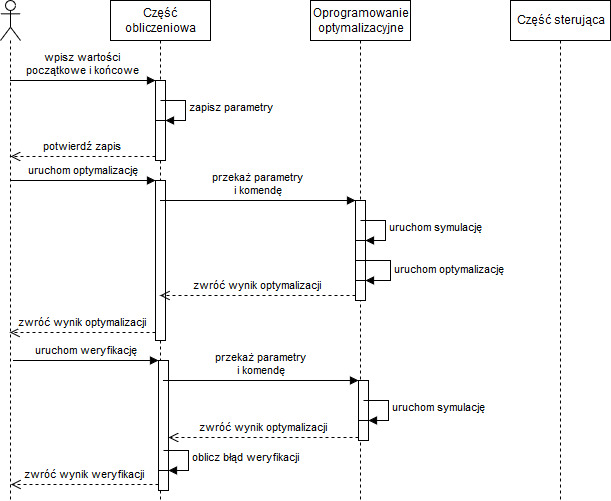
\includegraphics[width=\textwidth]{Grafika/communication-toc}
    \caption{Diagram sekwencji ilustrujący akcję obliczenia sterowania czasooptymalnego. Źródło: własne.}\label{fig:comm-toc}
\end{figure}

\begin{figure}[hpt]
    \centering
    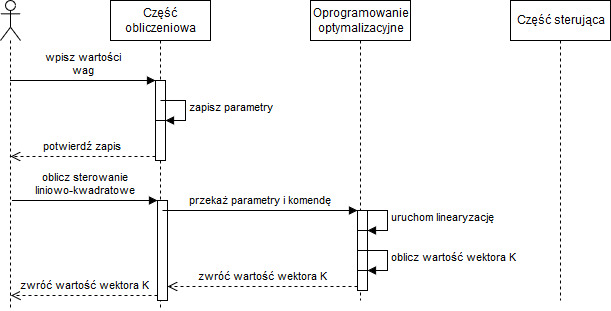
\includegraphics[width=\textwidth]{Grafika/communication-lqr}
    \caption{Diagram sekwencji ilustrujący akcję obliczenia sterowania liniowo-kwadratowego. Źródło: własne.}\label{fig:comm-lqr}
\end{figure}

\begin{figure}[hpt]
    \centering
    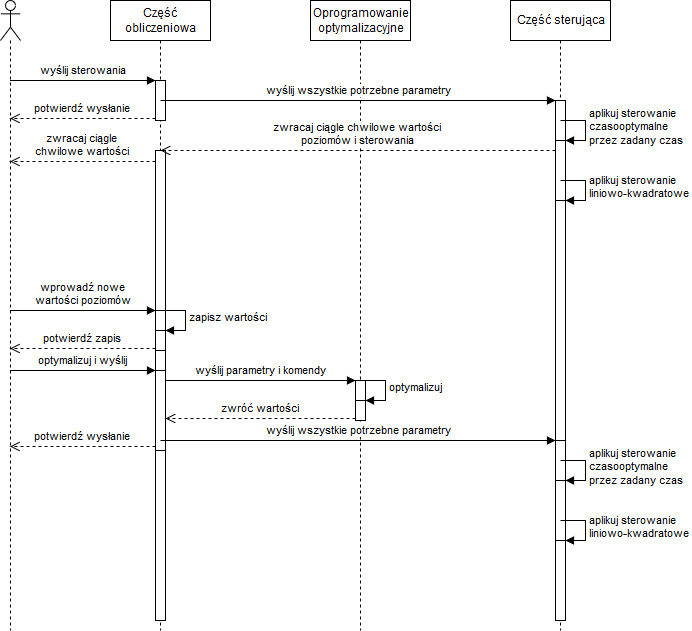
\includegraphics[width=\textwidth]{Grafika/communication-between-levels}
    \caption{Diagram sekwencji ilustrujący akcję wysyłania sterowań. Źródło: własne.}\label{fig:comm-send}
\end{figure}

\chapter{Opis oprogramowania}
\label{cha:software}

W niniejszym rozdziale znajduje się opis napisanej na potrzebny tej pracy aplikacji realizujące postawione w temacie zadanie. W poszczególnych podrozdziałach opisano wszystkie techniczne aspekty mające wpływ na ostateczny kształt obu poziomów utworzonego oprogramowania.

\section{Część obliczeniowa (,,wyższego poziomu'')}
\label{sec:czesc-wyzsza}

Aby zapewnić jak najlepszą realizację zadań postawionych przed częścią obliczeniową, należało wybrać odpowiednie oprogramowanie używane przez ten poziom aplikacji. Przyjęto dwa podstawowe założenia co do niego:
\begin{itemize}
    \item powinna być napisana w języku programowania Python,
    \item powinna używać biblioteki Tango Controls jako swojej podstawy.
\end{itemize}

Pierwsze założenie zostało przyjęte ze względu na niewątpliwe zalety tego języka. Jest on mocno zorientowany na programowanie obiektowe, posiada przejrzystą, nieskomplikowaną składnię oraz, jako język interpretowany, umożliwia szybkie prototypowanie i korzystanie z interaktywnego wiersza poleceń.

Dodatkowo jest to język dostępny w całości na otwartej licencji, a społeczność skupiona wokół niego dostarcza wielu bibliotek ogólnego i szczególnego zastosowania, które również często są otwartym oprogramowaniem. Podjęto w związku z tym próbę znalezienia wśród tych bibliotek takich, które byłyby pomocne w rozwiązywaniu zagadnień optymalizacji dynamicznej - więcej na ten temat w sekcji \ref{sub:czesc-wyzsza-wybor}.

Drugie założenie zostanie wyjaśnione w kolejnej sekcji.

%-------------------------------------------------
\subsection{Opis systemu Tango Controls}
\label{sub:czesc-wyzsza-tango}

Tango Controls to zestaw narzędzi służący do zarządzania rozproszonymi systemami sterowania umożliwiający przyłączanie dowolnych urządzeń oraz fragmentów oprogramowania do jednej magistrali programowej. Jest on również dystrybuowany na otwartej licencji (tzw. słabszej powszechnej licencji publicznej GNU - ang. \emph{Lesser GNU Public Licence} - w wersji 3) i utrzymywany przez konsorcjum placówek naukowych z całej Europy (więcj informacji w \cite{TangoWebsite}).


\subsubsection{Ogólne założenia systemu}
Początki tego oprogramowania sięgają roku 1999, kiedy to w Europejskim Ośrodku Synchrotronu Atomowego w Grenoble podjęto próbę implementacji nowego systemu pozwalającego na połączenie wszystkich urządzeń jedną magistralą programową i zaczęto pracę nad jej uogólnieniem, aby mogła przyjąć dowolny sprzęt, który tylko będzie miał napisany odpowiedni do niej sterownik. Osiągnięto ten cel dzięki użyciu odpowiedniej technologii komunikacyjnej (oryginalnie implementacji architektury CORBA, od wersji 7 również biblioteki ZeroMQ) oraz zastosowaniu własnego protokołu oraz ogólnej przestrzeni adresowej dla wszystkich urządzeń w systemie. Zastosowano tutaj również podejście ,,klient - serwer'', a więc istnieje wyraźne rozgranicznie między interfejsem dla klienta (aplikacji pobierającej dane z systemu) oraz serwera (aplikacji dostarczającej dane). Dostępne są 3 tryby komunikacji między klientami a serwerami:
\begin{itemize}
    \item synchroniczny,
    \item asynchroniczny,
    \item zdarzeniowy.
\end{itemize}

Przyłączanie nowego sprzętu do tego systemu opiera się na zasadzie opakowywania istniejącego kodu służącego do komunikacji z nim kodem realizującym operacje związane z systemem Tango Controls. W związku z tym, że jednym z podstawowych założeń tego systemu jest obiektowość, to opakowanie będzie miało postać \emph{klasy urządzeń}.
Dzięki temu przejmuje on wszystkie zalety (oraz pułapki) programowania obiektowego: możliwość dziedziczenia między klasami, co ułatwia utrzymywanie hierarchicznej struktury pisanego oprogramowania, jak i możliwość współdzielenia bardziej ogólnych klas między różnymi systemami, które korzystają z Tango Controls. W szczególności wszystkie klasy muszą dziedziczyć po bazowej klasie - \emph{Device}.

\subsubsection{Urządzenia i ich serwery}
Podstawowym pojęciem opisywanego systemu jest \emph{urządzenie}, które jest obiektem w sensie programistycznym (instancją klasy danego typu urządzeń). Może to być:
\begin{itemize}
    \item logiczna abstrakcja istniejącego fizycznie sprzętu, niezależnie od tego, czy jest to jeden prosty czujnik, czy bardziej skomplikowane urządzenie z własnym HMI (ang. \emph{Human-Machine Interface}: interfejs człowiek-maszyna),
    \item logiczna abstrakcja grupy urządzeń, również niezależnie od ich stopnia skomplikowania,
    \item fragment oprogramowania - mówi się wtedy o czysto programowym urządzeniu.
\end{itemize}

Definicja przestrzeni adresowej systemu zakłada, że każde urządzenie w systemie ma nazwę składającą się z 3 członów przedzielonych prawymi ukośnikami (,,/''):
\begin{itemize}
    \item domeny,
    \item rodziny,
    \item członka.
\end{itemize}
Przykładowa nazwa wygląda następująco: \texttt{sys/tg\_test/1}.

Dodatkowo podając nazwę urządzenia, można również podać adres bazowy systemu, czyli adres i port, na którym można nawiązać komunikację TCP/IP z urządzeniem zarządzającym dostępem do warstwy persystencji systemu - bazy danych MySQL. Tam przechowywane są informacje na temat urządzeń kiedykolwiek uruchomionych w systemie. Taki adres bazowy systemu określa się jako zmienną środowiskową w systemie operacyjnym o nazwie \texttt{TANGO\_HOST}. Określenie takiej pary adresu i portu jednoznacznie definiuje, z którym systemem zarządzanym przez Tango Controls klient się chce połączyć. Uzupełniona o nią (i o nazwę protokołu) przykładowa nazwa urządzenia wygląda następująco: \texttt{tango://tango-host.org:10000/sys/tg\_test/1}.

Urządzenia systemu Tango są grupowane w \emph{serwery urządzeń} - procesy w systemie operacyjnym, które przy swoim starcie pytają warstwy persystencji o to, jakie urządzenia mają uruchomić. Każdy serwer urządzeń ma określony zestaw klas urządzeń, których instancjami może zarządzać: uruchamiać je, edytować, wyłączać, kasować itp. Umożliwia on również włączenie odpytywania konkretnego elementu interfejsu urządzenia z okresem zadanym w milisekundach. Proponuje się rozróżnienie na klasę urządzeń i typ serwera urządzeń, aby uniknąć nieścisłości. Każdy serwer jest również obiektem klasy urządzeń \emph{DServer}, a jego typ określa to, jakimi klasami urządzeń dysponuje.

Na interfejs urządzenia składają się cztery typy pól w klasie tego urządzenia:
\begin{enumerate}
    \item Atrybuty (ang. \emph{attributes}) - reprezentują wielkości fizyczne, zmieniające się w czasie działania urządzenia. Muszą mieć zdefiniowany typ (jeden z podstawowych typów danych numerycznych lub ciągu znaków) oraz wymiar (Tango Controls obsługuje atrybuty skalarne, wektorowe i macierzowe). Każde urządzenie musi mieć przynajmniej 2 atrybuty: stan i status (testowy opis tego, co się dzieje z urządzeniem). Przykładowy atrybut urządzenia będącego odwzorowaniem silnika krokowego w systemie Tango to pozycja (zmiennoprzecinkowa wartość skalarna) lub stan wyłączników krańcowych (dwuelementowy wektor wartości logicznych).
    
    \item Strumienie (ang. \emph{pipe} - pozwalają na przesyłanie dowolnego typu surowych danych do urządzenia lub na jego zewnątrz. Dla każdej ich paczki trzeba jednak określić ten typ przed transmisją. Mogą być jedno- lub dwukierunkowe. Jest to nowy typ pola w klasach urządzeń, obecny od wersji 9.
    
    \item Komendy (ang. \emph{commands})- będące operacjami, których wykonanie urządzenie umożliwia. Mogą być wywoływane z maksymalnie jednym argumentem wejściowym i również tylko jeden argument wyjściowy mogą zwracać. Przykładem komendy urządzenia będącego logiczną abstrakcją silnika krokowego jest operacja bazowania - znalezienie określonej pozycji sprzężonego enkodera i wyzerowanie rejestru położenia.
    
    \item Właściwości (ang. \emph{properties}) - zawierające statyczną konfigurację urządzenia. Jako jedyne są przechowywane w bazie danych, skąd serwer urządzeń przy starcie pobiera ich wartości.
\end{enumerate}

\begin{figure}[tph]
    \centering
    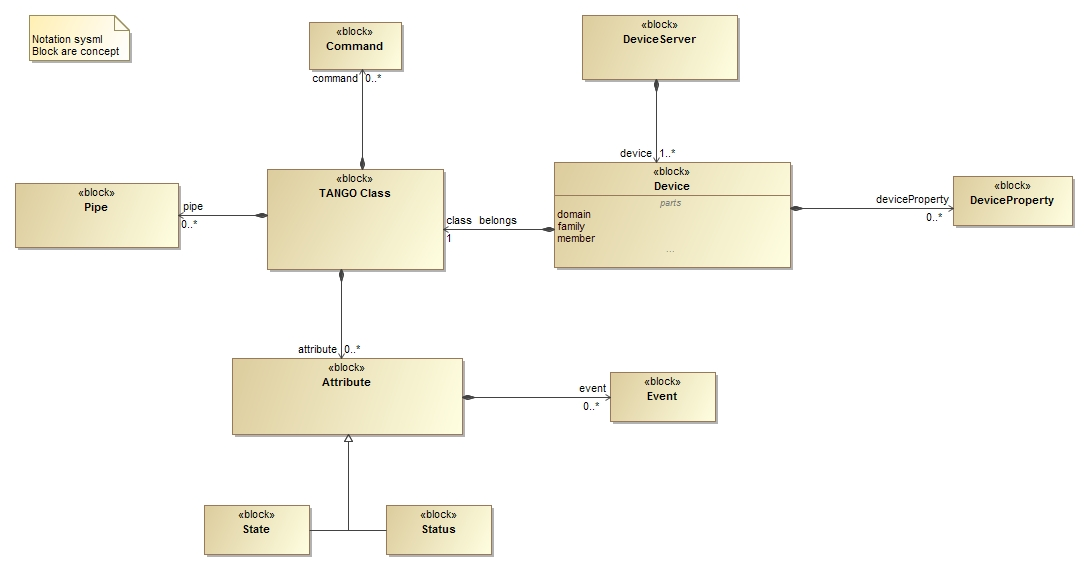
\includegraphics[width=\textwidth]{Grafika/tango_model}
    \caption{Uproszczony model obiektów w systemie Tango Controls. Źródło: \cite{TangoDocs}.}
    \label{fig:tango-model}
\end{figure}

Klasa urządzeń może zawierać definicję maszyny stanów, która opisuje warunki przejść między dowolnymi z 14 dostępnych stanów. Są w tym zbiorze ogólne stany opisujące poprawne działanie urządzenia (INIT, ON, OFF, STANDBY, RUNNING, MOVING), błędy w funkcjonowaniu (ALARM, FAULT, DISABLE), takie nadające się tylko dla określonych typów sprzętu (OPEN, CLOSE, INSERT, EXTRACT) oraz stan nieustalony (UNKNOWN). Maszyna stanów może również ograniczać dostęp do innych elementów interfejsu urządzenia (atrybutów i komend) na podstawie tego, w jakim stanie ono się znajduje.

Wszystkie opisane wyżej pojęcia oraz relacje między nimi zostały przedstawione na diagramie \ref{fig:tango-model}. Znajduje się tam klasa urządzeń (ang. \emph{Device Class}, \emph{TANGO Class}), która definiuje elementy interfejsu urządzeń będących jej instancjami (atrybuty, komendy i strumienie).
Na schemacie zostały dodatkowo oznaczone zdarzenia (ang. \emph{Events}), których każdy atrybut może wysyłać 3 typy: okresowe, archiwizacji i zmiany. Dodatkowo zaznaczono, że urządzenie musi posiadać atrybuty stanu i statusu.
Urządzenie jest obiektem takiej klasy i należy do serwera urządzeń (ang. \emph{Device Server}). Każde dodatkowo ma konkretne wartości właściwości przechowywane w bazie danych systemu Tango.

\subsubsection{Interfejs programistyczny systemu}
Specyfikacja Tango Controls definiuje API (ang. \emph{Application Programming Interface}: interfejs programowania aplikacji), do którego jest dostęp w różnych językach programowania na wielu systemach operacyjnych (m.in.: różne dystrybucje systemu Linux, Windows, Mac OS oraz Solaris). Jest on dokładnie opisany w dokumentacji dostępnej w \cite{TangoDocs}.

Tabela \ref{tab:tango-implementations} podsumowuje wszystkie możliwe technologie, z których można korzystać, aby łączyć się z systemem zarządzanym przez Tango Controls. Informacje te są też przedstawione w graficznej formie na rys. \ref{fig:tango-bindings}.

Oprócz tego istnieje też bogaty zestaw narzędzi służących do zarządzania systemem, nadzorowania go, tworzenia interfejsów graficznych oraz realizowania innych usług wymaganych w rozproszonym systemie sterowania (np. archiwizacji, zbierania logów czy automatycznej konfiguracji).

\begin{table}[hpt]
    \centering
    \begin{tabular}{|c|c|c|}
        \hline 
        \textbf{Język} & \textbf{Typ implementacji} &\textbf{Co umożliwia} \\ 
        \hline 
        C++ & pełna & klient i serwer \\ 
        \hline 
        Java & pełna & klient i serwer \\ 
        \hline 
        Python & opakowanie do implementacji w C++ & klient i serwer \\ 
        \hline 
        C & opakowanie do implementacji w C++ & klient \\ 
        \hline 
        LabView & implementacja pomocnicza w języku C++ & klient i serwer \\ 
        \hline 
        MATLAB/Octave & tylko warstwa komunikacyjna w języku C++ & klient \\ 
        \hline 
        IgorPro & tylko warstwa komunikacyjna w języku C++ & klient \\ 
        \hline 
        Panorama & wtyczka do aplikacji & klient \\ 
        \hline 
        JavaScript & tylko warstwa komunikacyjna z użyciem protokołu REST & klient \\ 
        \hline 
    \end{tabular}
    \caption{Podsumowanie języków programowania, w których istnieje możliwość połączenia z systemem Tango Controls. Źródło: \cite{TangoWebsite}.}
    \label{tab:tango-implementations}
\end{table}

\begin{figure}[ht]
    \centering
    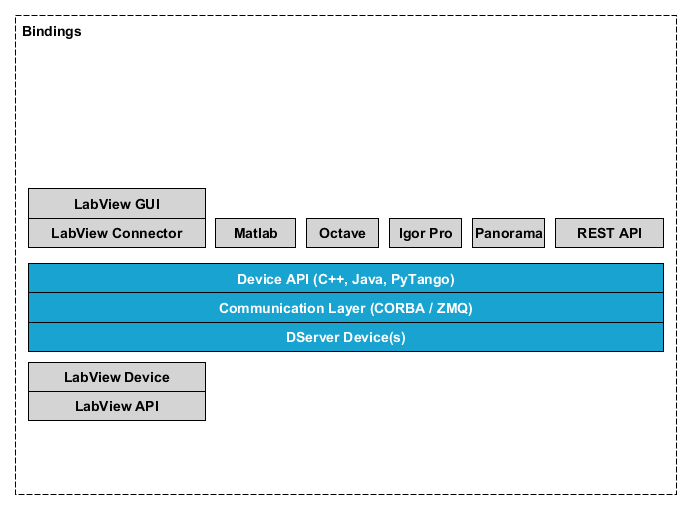
\includegraphics[width=\textwidth]{Grafika/tango_bindings_map1_1}
    \caption{Mapa wtyczek do systemu Tango Controls. Źródło: \cite{TangoDocs}.}\label{fig:tango-bindings}
\end{figure}

W związku ze wszystkimi opisanymi cechami uznano Tango Controls za odpowiednią bibliotekę do oparcia na niej części obliczeniowej aplikacji stanowiącej podstawę niniejszej pracy magisterskiej.


%-------------------------------------------------
\subsection{Architektura klasy urządzeń systemu Tango}
\label{sub:czesc-wyzsza-klasa}

Architektura systemu Tango Controls wymusiła pewne decyzje co do struktury tej części aplikacji. Zdecydowano, że będzie ona napisana jako klasa urządzeń, która określa interfejs dla wszystkich operacji wymaganych do spełnienia zadań postawionych przed tym poziomem aplikacji w podrozdziale \ref{sec:podzial-zadan}. Nie zdecydowano się na podział zadań na mniejsze klasy urządzeń komunikujące się ze sobą. Przyjęto, że prostsza struktura z jedną klasą ułatwi użycie napisanego kodu w przyszłości, np. w formie części zajęć laboratoryjnych.

\subsubsection{Interfejs dla systemu Tango}

Określając interfejs dla systemu Tango, przyjęto założenie, że wszystkie parametry statyczne modelu matematycznego powinny być również statyczną konfiguracją urządzenia, a więc należy opisać je jako jego właściwości. Głównym powodem przyjęcia takiej reguły jest fakt, iż w czasie działania - realizacji sterowania optymalnego - te wielkości nie będą się zmieniać.
Parametry dynamiczne, czyli takie, które zmieniają się między uruchomieniami algorytmów optymalizacyjnych, powinny zostać opisane jako atrybuty urządzenia.
Wszystkie dostępne akcje na modelu matematycznym zostały zaimplementowane jako komendy. Dodano tam również wszystkie akcje opisane w podrozdziale \ref{sec:komunikacja}.

Poniższa lista zawiera wszystkie istotne dla użytkownika elementy interfejsu systemu Tango urządzenia realizującego zadania wyższego poziomu aplikacji. Każdy z nich jest pokrótce opisany.

\begin{enumerate}
    \item Właściwości:
    \begin{enumerate}
        \item \emph{IPOPTTolerance} - tolerancja błędów oprogramowania do rozwiązywania zagadnień algebry liniowej (więcej o wpływie na działanie optymalizacji w sekcji \ref{sub:opt-dokladnosc}).
        \item \emph{ModelFile} - nazwa pliku z modelem dla oprogramowania do optymalizacji (więcej w sekcji \ref{sub:czesc-wyzsza-wybor}).
        \item \emph{MaxControl} - górne ograniczenie sterowania.
        \item \emph{Tank*Outflow} - opory wypływu ze zbiorników $C_{i}$. Dane jako 3 osobne właściwości - w miejscu * jest liczba 1, 2 lub 3.
        \item \emph{Tank*FlowCoeff} - współczynniki wypływu ze zbiorników $\alpha_{i}$. Dane j.w.
        \item \emph{SimulationFinalTime} - czas symulacji używanej w celu inicjalizacji algorytmu optymalizacji (więcej o tym procesie w sekcji \ref{sub:opt-init}.
        \item \emph{TCPServerEnabled} - wartość logiczna zawierająca informację o tym, czy urządzenie ma uruchomić serwer TCP w celu komunikowania się z aplikacją niższego poziomu.
        \item \emph{TCPServerAddress} - para adres i port (przedzielone dwukropkiem). Pod tym adresem serwer TCP będzie nasłuchiwał przychodzących połączeń.
    \end{enumerate}
    \item Atrybuty (nie umożliwiają zapisu, chyba że zaznaczono inaczej):
    \begin{enumerate}
        \item \emph{H*Current} - zawierają aktualne poziomy wody w zbiornikach odebrane od aplikacji niższego poziomu. Dane jako 3 osobne atrybuty - w miejscu * jest liczba 1, 2 lub 3.
        \item \emph{H*Initial} - zawierają początkowe wartości poziomów dla optymalizacji dynamicznej. Dane j.w., możliwy zapis.
        \item \emph{H*Final} - zawierają końcowe wartości poziomów dla optymalizacji dynamicznej. Dane j.w., możliwy zapis.
        \item \emph{H*Simulated} - zawierają wektory przebiegu poziomów w zbiornikach uzyskane w symulacji. Dane j.w.
        \item \emph{OptimalH*} - zawierają wektory przebiegu poziomów w zbiornikach uzyskane w czasie optymalizacji (wyznaczania sterowania czasooptymalnego). Dane j.w.
        \item \emph{OptimalTime} - liczba będąca wartością wskaźnika jakości uzyskaną w procesie wyznaczania sterowania czasooptymalnego.
        \item \emph{SimulationTime} - wektor wartości czasu uzyskany w czasie symulacji potrzebny w celu rysowania przebiegów symulacyjnych \emph{H*Simulated}.
        \item \emph{OptimalControl} - wektor zawierający sterowanie czasooptymalne.
        \item \emph{ControlCurrent} - zawiera aktualną wartość sterowania odebraną od aplikacji niższego poziomu.
        \item \emph{SwitchTimes} - wektor zawierający czasy przełączeń po normalizacji sterowania czasooptymalnego.
        \item \emph{Q} - macierz 3 na 3 zawierająca wagi poziomów do zagadnienia liniowo-kwadratowego. Możliwy zapis.
        \item \emph{R} - wartość wagi sterowania do zagadnienia liniowo-kwadratowego. Możliwy zapis.
        \item \emph{K} - wektor współczynników regulatora liniowo-kwadratowego.
        \item \emph{VerificationError} - wartość błędu weryfikacj (więcej o jego wyznaczaniu w podrozdziale \ref{sec:sym-wer}).
        \item Dostępne stany:
        \begin{enumerate}
            \item OFF - model początkowy jest niewczytany.
            \item STANDBY - model początkowy jest wczytany, ale nie trwa żadna długa operacja.
            \item ON - trwa symulacja.
            \item RUNNING - trwa optymalizacja.
            \item ALARM - długa operacja się nie udała. W przypadku optymalizacji oznacza to, iż nie udało się znaleźć sterowania optymalnego. W przypadku weryfikacji, że zwróciła ona błąd (więcej na ten temat w sekcji \ref{sub:sym-wer-jmodelica}).
        \end{enumerate}
    \end{enumerate}
    \item Komendy:
    \begin{enumerate}
        \item \emph{LoadInitialModel} - wczytuje model początkowy służący do inicjalizacji symulacji i optymalizacji.
        \item \emph{ResetModel} - resetuje wczytany model początkowy.
        \item \emph{GetEquilibriumFromControl} - przyjmuje wartość sterowania i na jej podstawie wylicza punkt równowagi, a następnie ustawia odpowiednie wartości poziomów końcowych.
        \item \emph{RunSimulation} - uruchamia symulację, a po jej zakończeniu ustawia wartości zmiennych symulacyjnych.
        \item \emph{RunVerification} - uruchamia symulację, a po jej zakończeniu ustawia wartości zmiennych symulacyjnych oraz wylicza błąd weryfikacji.
        \item \emph{Optimise} - uruchamia procedurę optymalizacji, a następnie ustawia wartości poziomów optymalnych, sterowania optymalnego i osiągniętego czasu. Przyjmuje jeden argument - wartość logiczną, która określa, czy jako wartości początkowych powinna użyć aktualnych poziomów wody w zbiornikach. Jeśli tak się dzieje, to natychmiast po zakończeniu optymalizacji uruchamia komendę \emph{SendControl}.
        \item \emph{NormaliseOptimalControl} - przeprowadza operację normalizacji sterowania czasooptymalnego (więcej na ten temat w sekcji \ref{sub:opt-dokladnosc}) i ustawia wartości czasów przełączeń.
        \item \emph{SendControl} - sprawdza, czy są gotowe wartości do wysłania do aplikacji niższego poziomu, czyli czasy przełączeń i wartości wektora $K$ (jeśli nie są gotowe, uruchamia komendę \emph{GetLQR}), a następnie wysyła je do serwera TCP.
        \item \emph{GetDataFromDirectControl} - odbiera od serwera TCP dane od aplikacji sterowania bezpośredniego. Jest odpytywana standardowo co 50 milisekund. Ustawia aktualne poziomy i sterowanie.
        \item \emph{GetLQR} - uruchamia procedurę linearyzacji i wyliczania parametrów regulatora liniowo-kwadratowego. Ustawia wartości wektora K.
        \item \emph{GetEigenvaluesFromClosedLoopWithLQR} - zwraca w formie tekstowej wartości własne macierzy $A - BR^{-1}B^{T}K$ opisującej układ zamknięty sterowany regulatorem liniowo-kwadratowym.
    \end{enumerate}
\end{enumerate}

%TODO: Lista komend, właściwości i atrybutów

\subsubsection{Problem dostępności interfejsu}

%Wątki vs procesy w Pythonie
%Propozycja uniwersalnego rozwiązania długich funkcji w DS Tango

%-------------------------------------------------
\subsection{Wybór pakietu do optymalizacji dynamicznej}
\label{sub:czesc-wyzsza-wybor}

Podstawowym elementem istotnym dla powodzenia takiego zadania był wybór pakietu realizującego operacje optymalizacji dynamicznej. Istnieje na rynku kilka płatnych bibliotek bądź pakietów oprogramowania, które są w stanie rozwiązywać tego typu problemy (np. MATLAB, Mathematica itp.), ale postanowiono poszukać darmowego odpowiednika, który posiadałby interfejs w języku programowania Python (w związku z ogólnymi założeniami co do struktury tej części aplikacji).


\subsubsection{Opis pakietu ACADO}


\subsubsection{Opis pakietu Modelica}


%-------------------------------------------------
\subsection{Środowisko testowe części obliczeniowej}
\label{sub:czesc-wyzsza-docker}

\section{Część realizująca sterowanie bezpośrednie (,,niższego poziomu'')}
\label{sec:czesc-nizsza}

Ze względu na dostępność sprzętu służącego do sterowania fizycznym układem zbiorników, wybór technologii mogącej stanowić podstawę niższego poziomu aplikacji był ograniczony do dwóch możliwości.

Stanowisko laboratoryjne jest wyposażone w komputer, który za pomocą karty przemysłowej RTDAC/PCI komunikuje się z układem czujników i pompą. Komputer komunikuje się z kartą za pomocą pakietu MATLAB/Simulink i to właśnie jest pierwsza opcja oprogramowania do komunikacji z urządzeniami wykonawczymi.

Alternatywnie, można skorzystać ze sterownika PLC firmy GE Fanuc z serii Versa Max. Wybrano pierwszą możliwość ze względu na fakt, iż pakiet MATLAB/Simulink umożliwia symulację modelu zbiorników, w której można przeprowadzić dodatkową weryfikację sterowania czasooptymalnego obliczonego przez aplikację wyższego poziomu.

%-------------------------------------------------
\subsection{Pakiet MATLAB/Simulink jako narzędzie realizujące sterowanie bezpośrednie}
\label{sub:czesc-nizsza-matlab}

Oprogramowanie firmy Mathworks jest jedynym z najbardziej popularnych środowisk do wykonywania obliczeń i analizy ich wyników, tworzenia interfejsów użytkownika, symulacji i sterowania urządzeniami zewnętrznymi. Zawiera ono zestaw metod numerycznych realizujących szerokie spektrum zadań z różnych obszarów inżynierii. Definiuje również własny język oprogramowania zbliżony do języka Java cechujący się podejściem obiektowym i prostym zapisem operacji macierzowych.

Pakiet Simulink, będący częścią oprogramowania MATLAB, umożliwia opis układów fizycznych przy pomocy języka graficznego, którego modele składają się z bloczków opisujących operacje i połączeń między nimi. Daje dostęp do całkowania takich modelów przy użyciu różnych metod, zarówno z czasem ciągłym, jak i dyskretnym. Poza tym można używać go do realizacji sterowania bezpośredniego albo przez bezpośrednie połączenie z urządzeniami wykonawczymi, albo przez generację kodu opisującego modele w języku C lub VHDL na odpowiednie platformy sprzętowe.
Niestety, to oprogramowanie jest dostępne tylko na płatnych licencjach różnego typu.

Istnieje wiele przykładów zastosowań pakietu MATLAB/Simulink w celu realizacji zadań sterowania czasooptymalnego (np. \cite{Trawinski2011}), ale ze względu na założoną z góry hybrydowość aplikacji opisywanej w niniejszej pracy, nie zdecydowano się na wykorzystanie go również w takim celu.

\begin{figure}
    \centering
    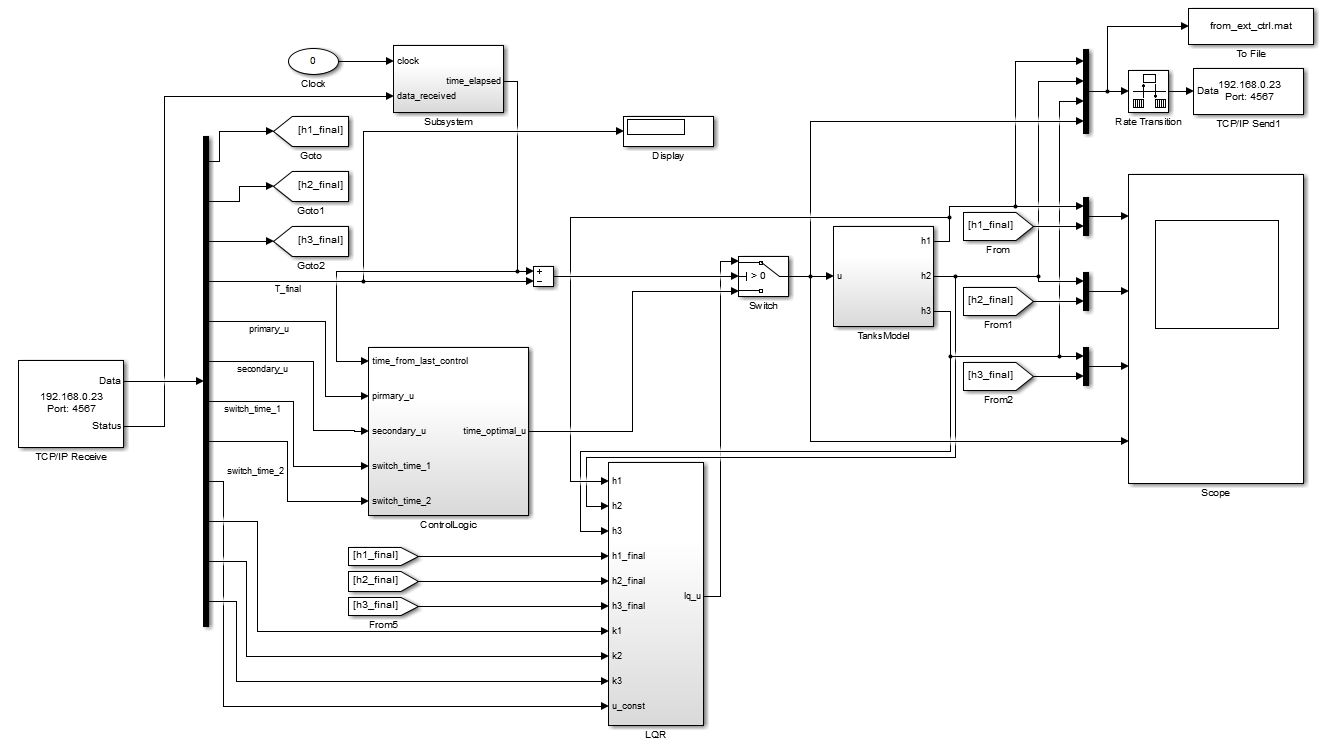
\includegraphics[scale=0.65,angle=90]{Grafika/simulink_model}
    \caption{Model niższego poziomu aplikacji w programie Simulink. Źródło: własne.}
    \label{fig:simulinkmodel}
\end{figure}

Przygotowano model w programie Simulink, pokazany na rys. \ref{fig:simulinkmodel}, który stanowi niższy poziom aplikacji. Zawiera on następujące komponenty:
\begin{itemize}
    \item odbiór danych z wyższego poziomu aplikacji za pomocą protokołu TCP,
    \item układ wyznaczający czas rozpoczęcia realizacji zadania sterowania czasooptymalnego,
    \item układ wyznaczający aktualną wartość sterowania czasooptymalnego na podstawie czasów przełączeń,
    \item układ wyznaczający sterowanie liniowo-kwadratowe,
    \item blok wybierający sterowanie do zaaplikowania w modelu (kryterium przełączenia jest czas będący wartością wskaźnika jakości w zadaniu czasooptymalnym),
    \item podsystem zawierający definicję modelu układu zbiorników,
    \item wysyłanie danych uzyskanych w symulacji (aktualnych poziomów wody w zbiornikach i sterowania) do wyższego poziomu aplikacji i zapisywanie ich do pliku w celu późniejszej analizy,
    \item blok pozwalający na rysowanie wykresów trajektorii systemu w czasie symulacji.
\end{itemize}

Przeprowadzone testy komunikacji między poziomami aplikacji wykazały, że serwer urządzeń systemu Tango Controls, będący wyższym jej poziomem, nie jest w stanie obsłużyć wysyłanych w każdym kroku symulacji danych. Zastosowano więc blok wyzwalający wysyłanie z mniejszą częstotliwością. Dobrano eksperymentalnie wartość 100 ms jako okres wysyłania, ponieważ stwierdzono, że dynamika układu jest stosunkowo wolno zmienna, a więc taki okres nie spowoduje większych błędów w obliczaniu sterowania czasooptymalnego przez część obliczeniową aplikacji.

\chapter{Badania symulacyjne}
\label{cha:symulacja}

\section{Optymalizacja przy użyciu pakietu JModelica.org}
\label{sec:opt}

Podstawowym zadaniem wyższego poziomu aplikacji było przeprowadzenie optymalizacji w celu wyznaczenia sterowania czasooptymalnego. Jak wspomniano w sekcji \ref{sub:czesc-wyzsza-wybor}, wybrano do tego celu platformę JModelica.org.

%-------------------------------------------------
\subsection{Opis algorytmu optymalizacji dynamicznej}
\label{sub:opt-alg}

Algorytm wykorzystywany do optymalizacji dynamicznej można ogólnie opisać jako bezpośrednią metodę kolokacji. Polega ona na aproksymacji układu równań różniczkowych w dyskretnych chwilach czasu i konstrukcji na tej podstawie zadania programowania nieliniowego, zwykle o rzadkiej strukturze. Jest napisana w języku Python i używa biblioteki CasADi do wyznaczenia wartości pochodnych funkcji oraz oprogramowania IPOPT do obliczenia wynikowego zagadnienia programowania nieliniowego. Można z niej korzystać pod warunkiem, że model matematyczny nie zawiera nieciągłości (za: \cite{JModelicaUserGuide}). W związku z tym, że nieciągłość występuje w rozważanym modelu zbiorników dla zerowego poziomu w trzecim zbiorniku, należało unikać trajektorii zawierających ten punkt.

Programy rozwiązujące problemy NLP wykazują się dużo większą zbieżnością w przypadku, gdy dostarczy się im informacje o pochodnych pierwszego i drugiego rzędu (za: \cite{and+11mod11}). W związku z tym w użytym algorytmie użyto najpierw oprogramowania CasADi, aby ze skompilowanego modelu w języku Modelica wyznaczyć wartości tych pochodnych (w formie jakobianu), a następnie używa się metody elementów skończonych. Dzieli ona wyjściowy przedział czasowy na określoną liczbę przedziałów nazywanych elementami skończonymi i dostarcza aproksymacji nieznanych wartości sterowania i stanów systemu w określonej liczbie punktów kolokacji. Wpływ liczby elementów na jakość rozwiązania jest przedstawiony w sekcji \ref{sub:sym-wer-jmodelica}.
W każdym punkcie kolokacji zastosowano pakiet IPOPT, który rozwiązuje zadanie w postaci danej wzorem \ref{eq:opt-stat} za pomocą metody punktu wewnętrznego. Metoda ta wykorzystuje funkcję graniczną do poruszania się tylko wewnątrz zbioru dopuszczalnego, gdzie metodą Newtona szuka lokalnego minimum.

\begin{equation}\label{eq:opt-stat}
    \min\limits_{x \in [x_{l}, x_{u}]~ \land~ g_{l} \leq g(x) \leq g_{u}} f(x)
\end{equation}

Algorytm optymalizacyjny zwraca wektor sterowań oraz trajektorie układu w czasie będącym wartością wskaźnika jakości w tym zagadnieniu. Te wartości są prezentowane użytkownikowi jako odpowiednie atrybuty urządzenia systemu Tango Controls.

%-------------------------------------------------
\subsection{Inicjalizacja optymalizacji dynamicznej}
\label{sub:opt-init}

Kluczowym aspektem funkcjonowania algorytmów optymalizacji dynamicznej jest odpowiednie określenie punktu początkowego, czyli początkowej struktury sterowania i wygenerowanej przez nią trajektorii układu. Jest to zagadnienie szeroko opisywane w literaturze, m.in w \cite{Betts98}, \cite{Rao2010}, \cite{Korytowski2015}, \cite{cas+11ifac} oraz \cite{JModelicaUserGuide}.
Początkowo próbowano inicjalizować algorytm stałym sterowaniem, którego wartość jest niezależna od punktów początkowych i końcowych. Niestety, takie podejście okazało się błędne i nie udało się wyznaczyć żadnego sterowania optymalnego.

W związku z tym przyjęto następujący algorytm inicjalizacyjny:
\begin{itemize}
    \item dla każdej z trzech wartości poziomów docelowych wyznacz wartość sterowania ustalonego na podstawie odwrotności wzoru \ref{eq:model-steady-state} danego wzorem \ref{eq:steady-ctrls},
    \begin{equation} \label{eq:steady-ctrls}
    u_{i} = C_{i}h_{i}^{\alpha_{i}}
    \end{equation}
    \item wyznacz wartość średnią z trzech sterowań ustalonych, wyznaczonych w poprzednim kroku według wzoru \ref{eq:steady-ctrl}
    \begin{equation}\label{eq:steady-ctrl}
    u_{r} = \frac{1}{3} \cdot \sum_{i=1}^{3} u_{i}
    \end{equation}
    \item przeprowadź symulację z czasem końcowym podanym jako wartość właściwości \emph{SimulationFinaltime} (opisanej w sekcji \ref{sub:czesc-wyzsza-klasa}),
    \item podaj wyniki uzyskane w symulacji jako trajektorie inicjalizacyjne do algorytmu optymalizacji.
\end{itemize}

\begin{figure}[ht]
    \centering
    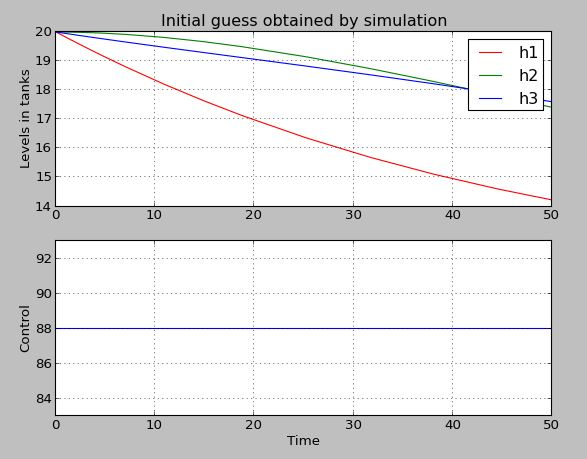
\includegraphics[scale=0.9]{Grafika/initial_guess}
    \caption{Przykładowa trajektoria początkowa dla algorytmu optymalizacji. Źródło: własne.}
    \label{fig:initialguess}
\end{figure}

Rysunek \ref{fig:initialguess} przedstawia przykładowe sterowanie ustalone i przebiegi zmiennych stanu uzyskane według powyższego algorytmu.

Tak dobrany algorytm inicjalizacji pozwolił osiągnąć zadowalające wyniki optymalizacji.


%-------------------------------------------------
\subsection{Uzyskana postać sterowania}
\label{sub:opt-ctrl-form}

W związku z tym, że użyte oprogramowanie jest w stanie dokonywać optymalizacji sterowania w układach nieliniowych, nie ma możliwości, aby ograniczyć postać sterowania tylko do postaci ,,bang-bang''. Sterowanie wyznaczane przez opisany wyżej algorytm optymalizacji jest wektorem o rozmiarze danym wzorem \ref{eq:ctrl-len}, gdzie $k$ to liczba punktów kolokacji, a $e$ to liczba elementów skończonych. Dodatkowy element wektora sterowania bierze się od wartości początkowej.

\begin{equation}\label{eq:ctrl-len}
l_{u} = k \cdot e + 1
\end{equation}

Niezależnie od tego okazało się, że sterowanie optymalne wyliczone przy pomocy pakietu JModelica.org ma często postać zbliżoną do ,,bang-bang'' ze spodziewaną liczbą dwóch przełączeń. Dowodzi to, iż założenie opisane w sekcji \ref{sub:toc-nonlnr} nie jest zawsze prawdziwe, ale może być zastosowane w pewnym podzbiorze zbioru stanów osiągalnych. Zauważono, że zwykle sprawdza się w przypadku niewielkiego oddalenia stanu docelowego optymalizacji od punktu równowagi systemu.

\begin{figure}[ht]
    \centering
    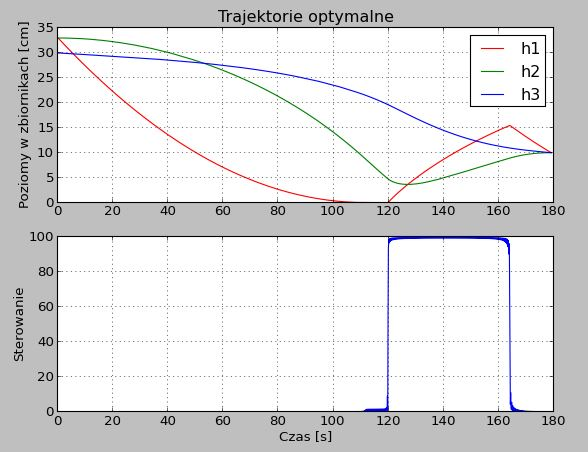
\includegraphics{Grafika/optimisation_example}
    \caption{Przykładowy wynik optymalizacji. Źródło: własne.}
    \label{fig:optimisationexample}
\end{figure}

Rysunek \ref{fig:optimisationexample} przedstawia przykładowe sterowanie optymalne oraz trajektorie układu przez nie wygenerowane. Można na nim zauważyć, że sterowanie nie jest dokładnie postaci ,,bang-bang'' (zbocze narastające zawiera punkt zmiany szybkości narastania), ale jest to niego zbliżone.

Przyjęto więc prostą metodę normalizacji sterowania do postaci ,,bang-bang'': każdemu punktowi powyżej połowy różnicy między ograniczeniami nałożonymi na sterowanie zostaje przypisana wartość maksymalna, a każdemu poniżej - minimalna. Jeśli występuje tylko jeden czas przełączenia, to dodaje się drugi w ostatniej chwili
Taka operacja pozwala wyznaczyć czasy przełączeń potrzebne niższemu poziomowi aplikacji, jeśli tylko sterowanie otrzymane z algorytmu optymalizacji ma spodziewaną strukturę. Przykład działania operacji normalizacji jest dany poniżej: przedstawiono sterowanie w postaci ,,surowej'' obliczonej przez algorytm optymalizacyjny i po normalizacji odpowiednio na rysunkach \ref{fig:ctrl-raw-example} i \ref{fig:ctrl-normalised-example}.

\begin{figure}[ht]
    \centering
    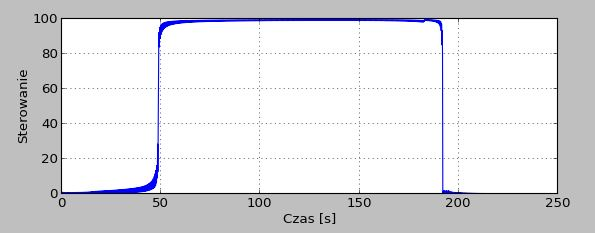
\includegraphics[width=\textwidth]{Grafika/ctrl_30_30_30-20_25_20-raw}
    \caption{Przykład sterowania ,,surowego'' otrzymanego w wyniku optymalizacji. Źródło: własne.}
    \label{fig:ctrl-raw-example}
\end{figure}

\begin{figure}[ht]
    \centering
    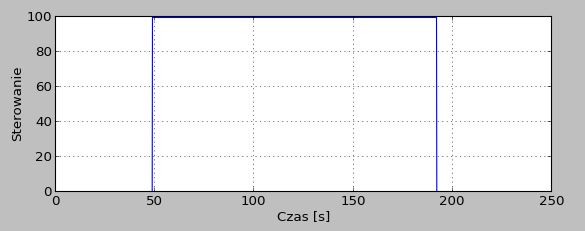
\includegraphics[width=\textwidth]{Grafika/ctrl_30_30_30-20_25_20-normalised}
    \caption{Przykład sterowania znormalizowanego. Źródło: własne.}
    \label{fig:ctrl-normalised-example}
\end{figure}

Niestety, tak prosty algorytm ma swoje wady. Przede wszystkim nie umożliwia wyznaczania tylko dwóch czasów przełączeń w przypadku, gdy postać sterowania jest bardziej skomplikowana. To ogranicza stosowanie całej aplikacji tylko do przypadków, w których da się to zrobić, ponieważ założono, że wyższy jej poziom wysyła zawsze 2 czasy przełączeń.


%-------------------------------------------------
\subsection{Dokładność wyznaczania rozwiązania}
\label{sub:opt-dokladnosc}

Jedynym parametrem, który wyznacza dokładność wyznaczania rozwiązania przez pakiet JModelica.org jest relatywna tolerancja zbieżności programu IPOPT, którą można ustawić we właściwości \emph{IPOPTTolerance} (opisanej w sekcji \ref{sub:czesc-wyzsza-klasa}). Domyślną wartością jest $10^{-5}$, która jednak okazała się zbyt mała dla opisywanego problemu i prowadziła do błędów zbieżności i niemożliwości wyznaczenia odpowiedniego rozwiązania. Dobrano doświadczalnie wartość $10^{-3}$ ze względu na fakt, iż w tym przypadku niemożliwość wyliczenia sterowania optymalnego zdarzała się relatywnie rzadko.

Dodatkowo wartość wspomnianej właściwości \emph{IPOPTTolerance} jest również wykorzystywana do sprawdzenia, czy rozwiązanie zwrócone przez algorytm optymalizacyjny jest poprawne. Sprawdza się, czy odległość między wartościami końcowymi trajektorii systemu a stanem docelowym jest mniejsza niż wartość tej właściwości.


\section{Symulacja i weryfikacja}
\label{sec:sym-wer}

Aby sprawdzić poprawność działania algorytmu optymalizacji dynamicznej, wykonano symulacje weryfikacyjne przy użyciu oprogramowania JModelica.org na wyższym poziomie aplikacji oraz środowiska MATLAB/Simulink na niższym.
W obu tych przypadkach błąd weryfikacji jest liczony według wzoru \ref{eq:ver-error}, gdzie $h_{i}^{s}(T)$ to wartość odpowiedniego poziomu po upływie czasu optymalnego uzyskana w symulacji, a $h_{i}^{f}$ to wartość docelowa tego poziomu.

\begin{equation}\label{eq:ver-error}
e_{wer} = \sum_{i=1}^{3} (h_{i}^{s}(T) - h_{i}^{f})^{2}
\end{equation}

Należy zwrócić uwagę na to, iż weryfikacja poprawności rozwiązania korzysta z innych danych, niż sprawdzenie dokładności rozwiązania opisane w sekcji \ref{sub:opt-dokladnosc}. Pierwsza procedura używa danych symulacyjnych uzyskanych po optymalizacji, a druga - danych pochodzących bezpośrednio z algorytmu optymalizacyjnego.

%-------------------------------------------------
\subsection{Weryfikacja przy użyciu pakietu JModelica.org}
\label{sub:sym-wer-jmodelica}

Po zakończeniu optymalizacji wyższy poziom aplikacji umożliwia przeprowadzenie symulacji weryfikacyjnej. Podaje się wtedy cały uzyskany wektor sterowania optymalnego (w postaci ,,surowej'' lub znormalizowanej) jako trajektorię wejściową do symulacji, a na koniec wylicza się błąd weryfikacji.

Poniżej przedstawiono 2 przykłady wykresów uzyskanych w czasie weryfikacji i porównano wartości błędów przy zastosowaniu sterowania w postaci ,,surowej'' oraz znormalizowanej.

\begin{figure}[htp]
    \centering
    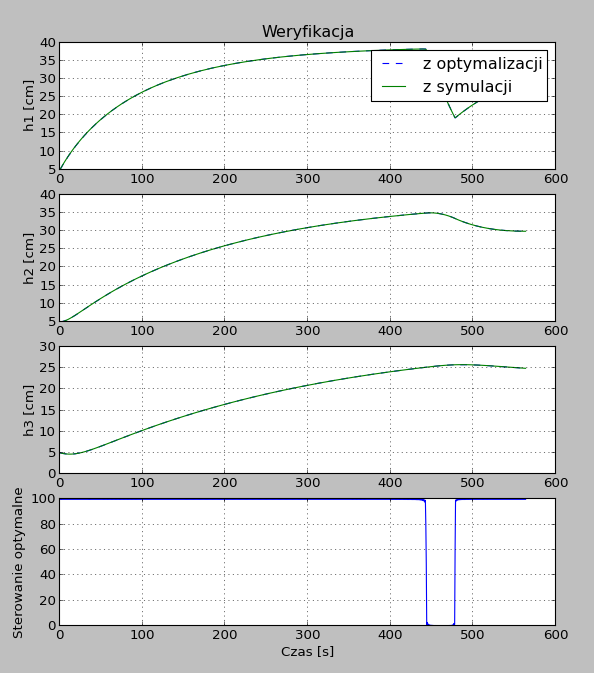
\includegraphics{Grafika/plot_5_5_6-30_30_25-raw-350}
    \caption{Przykładowa weryfikacja rozwiązania przy użyciu pakietu JModelica.org. Źródło: własne.}
    \label{fig:plot556-303035-raw-350}
\end{figure}

\begin{figure}[htp]
    \centering
    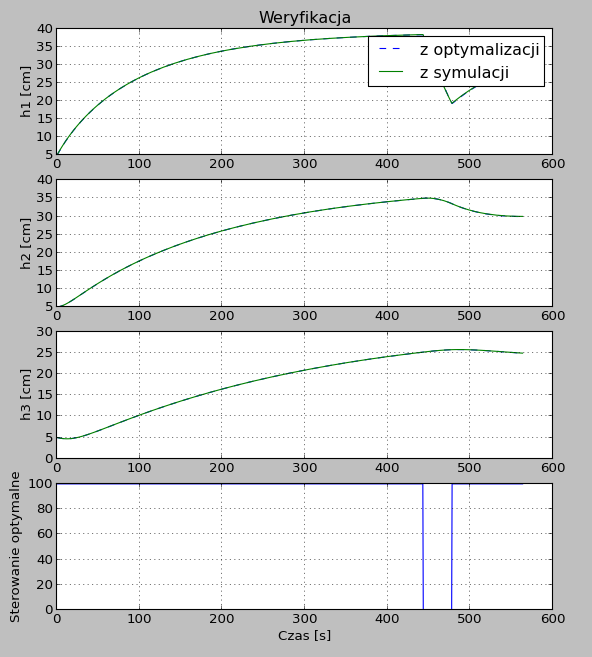
\includegraphics{Grafika/plot_5_5_6-30_30_25-normalised-350}
    \caption{Przykładowa weryfikacja po normalizacji sterowania. Źródło: własne.}
    \label{fig:plot556-303035-normalised-350}
\end{figure}

Pierwszy przykład to napełnianie zbiorników od poziomów $h_{1}^{0} = 5 cm, h_{2}^{0} = 5 cm, h_{3}^{0} = 6 cm$ do poziomów $h_{1}^{f} = 30 cm, h_{2}^{f} = 30 cm, h_{3}^{f} = 25 cm$. Sterowanie w postaci z algorytmu optymalizacji osiągnęło wartość błędu weryfikacji $e_{wer}^{s} = 0,0002$, a po znormalizowaniu: $e_{wer}^{n} = 0.002$. W tym przypadku sterowanie w postaci ,,surowej'' (przedstawione na rys. \ref{fig:plot556-303035-raw-350}) wizualnie nie różni się bardzo od sterowania znormalizowanego (pokazanego na rys. \ref{fig:plot556-303035-normalised-350}), ale nawet taka niewielka różnica może prowadzić do zwiększenia się błędu weryfikacji o rząd wielkości. Jest to jednak również związane z tym, iż pierwszy błąd jest bardzo niewielki i w czasie wielu prób rzadko uzyskiwano tak niewielkie wartości. W tej optymalizacji użyto 350 elementów skończonych.

\begin{figure}[htp]
    \centering
    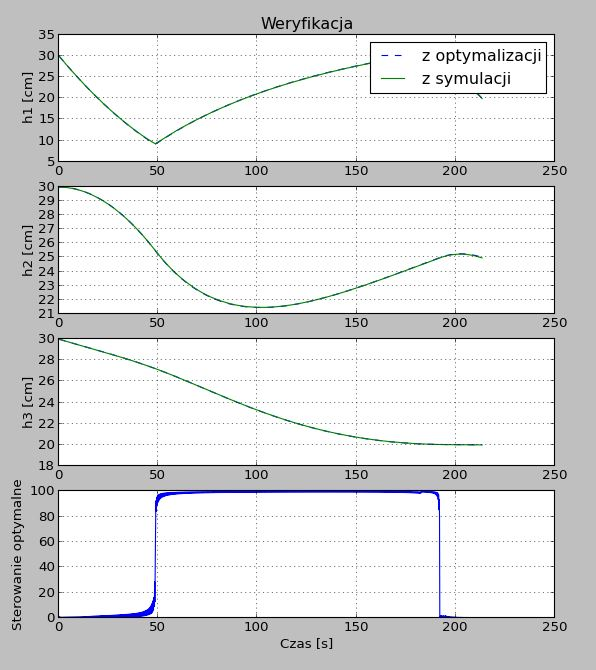
\includegraphics{Grafika/plot_30_30_30-20_25_20_raw_200}
    \caption{Druga przykładowa weryfikacja rozwiązania przy użyciu pakietu JModelica.org. Źródło: własne.}
    \label{fig:plot303030-202520raw200}
\end{figure}

\begin{figure}[htp]
    \centering
    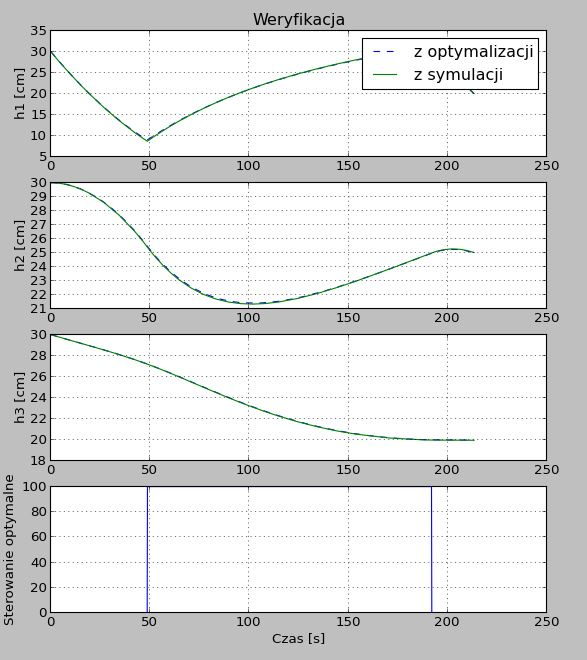
\includegraphics{Grafika/plot_30_30_30-20_25_20_normalised_200}
    \caption{Druga przykładowa weryfikacja po normalizacji sterowania. Źródło: własne.}
    \label{fig:plot303030-202520normalised200}
\end{figure}

Drugi przykład to upuszczanie niewielkiej ilości wody ze zbiorników od poziomów $h_{1}^{0} = 30 cm, h_{2}^{0} = 30 cm, h_{3}^{0} = 30 cm$ do $h_{1}^{f} = 20 cm, h_{2}^{f} = 25 cm, h_{3}^{f} = 20 cm$. Sterowanie w postaci ,,surowej'' osiągnęło wartość błędu weryfikacji $e_{wer}^{s} = 0,007$, a w postaci znormalizowanej: $e_{wer}^{n} = 0.019$. Tutaj różnica między błędami jest mniejsza niż w poprzednim przypadku, mimo bardziej skomplikowanej struktury sterowania wyznaczonego przez algorytm optymalizacyjny (pokazanego na rys. \ref{fig:plot303030-202520raw200}). Sterowanie znormalizowane zaprezentowano na rys. \ref{fig:plot303030-202520normalised200}. W tej optymalizacji użyto 200 elementów skończonych, więc trzeba to wziąć pod uwagę, porównując wartości błędów między oboma opisanymi przypadkami.


\subsubsection{Wpływ liczby elementów metody elementów skończonych na rozwiązanie}

W związku z tym, że zastosowana metoda przynosiła dobre rezultaty, lecz wartości błędu weryfikacji były dosyć duże (rzędu jednej dziesiątej), podjęto próbę zwiększenia liczby elementów skończonych i przeprowadzenia ponownej optymalizacji i weryfikacji. Odkryto, iż istotnie ma ono wpływ na wartość błędów weryfikacji, ale również na czas obliczeń.

Przeprowadzono więc eksperyment, który miał pokazać ten wpływ liczby elementów skończonych na błędy weryfikacji dla sterowania ,,surowego'' i znormalizowanego oraz czas obliczeń. Przyjęto zmianę tej liczby w przedziale 50 do 500 z krokiem 50 tak, aby uzyskać 10 punktów pomiarowych.

W pierwszym przypadku skorzystano z napełniania zbiorników od poziomu $h_{1}^{0} = h_{2}^{0} = h_{3}^{0} = 1 cm$ do $h_{1}^{f} = h_{2}^{f} = h_{3}^{f} = 15 cm$. Uzyskane wyniki przedstawiono na rys. \ref{fig:elementsinfluence1-15_50-500}. Zauważono, iż:
\begin{itemize}
    \item różnica absolutna i relatywna między błędem weryfikacji dla sterowania ,,surowego'' i znormalizowanego jest największa w przypadku najmniejszej rozważanej liczby elementów,
    \item prędkość zmniejszania się błędów
    \item wartości czasów obliczeń rosną najprawdopodobniej wielomianowo,
    \item należy stosować wartości liczby elementów z przedziału między 200 a 350, gdyż tam występuje najlepszy stosunek czasu obliczeń do wartości błędów.
\end{itemize}

\begin{figure}[ht]
    \centering
    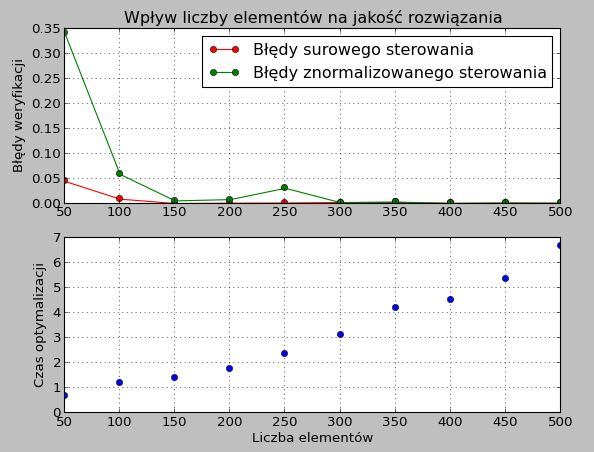
\includegraphics{Grafika/elements_influence_1-15_50-500}
    \caption{Wpływ liczby elementów skończonych na rozwiązanie. Źródło: własne.}
    \label{fig:elementsinfluence1-15_50-500}
\end{figure}

Przeprowadzono drugi eksperyment dla innych danych w celu weryfikacji powyższych wniosków. Tym razem skorzystano z napełniania zbiorników od poziomu $h_{1}^{0} = h_{2}^{0} = h_{3}^{0} = 10 cm$ do $h_{1}^{f} = h_{2}^{f} = h_{3}^{f} = 20 cm$. Wyniki pokazano na rys. \ref{fig:elementsinfluence10-2050-500}. Tym razem zaobserwowano, iż:
\begin{itemize}
    \item wartości błędów są zależne od warunków zadania - w tym przypadku błędy były około 2 razy większe,
    \item czasy obliczeń nie zachowują się tak regularnie, jak w powyższym przypadku i osiągają wartości o rząd wielkości większe, a więc również silnie zależą od warunków zadania,
    \item potwierdziła się hipoteza, iż należy wybierać wartości liczby elementów między 200 a 350.
\end{itemize}

\begin{figure}[ht]
    \centering
    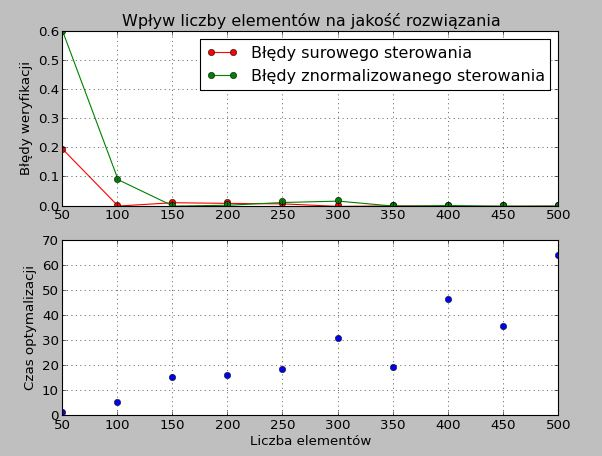
\includegraphics{Grafika/elements_influence_10-20_50-500}
    \caption{Drugi przykład wpływu liczby elementów skończonych na rozwiązanie. Źródło: własne.}
    \label{fig:elementsinfluence10-2050-500}
\end{figure}

\subsubsection{Problemy z błędną wartością pochodnej}

W przypadku niektórych wartości początkowych i końcowych oraz znalezionego dla nich sterowania optymalnego napotykano problem związany z tym, iż pakiet JModelica.org nie był w stanie obliczyć pochodnej jednego ze stanów w punkcie czasu niedługo po pierwszym przełączeniu. Rozwiązano go poprzez zwiększenie liczby elementów skończonych przy rozwiązywaniu danego zadania. Nie zaobserwowano takich problemów przy liczbie elementów powyżej 50.

%-------------------------------------------------
\subsection{Weryfikacja przy użyciu oprogramowania MATLAB/Simulink}
\label{sub:sym-wer-matlab}

%TODO: opisać wykresy i porównać z JModelicą

Symulację weryfikacyjną w programie MATLAB/Simulink przeprowadzono, łącząc oba poziomy aplikacji w całość i uruchamiając odpowiednie obliczenia. Zastosowano tam pewne uproszczenie: symulację uruchamiano dopiero po obliczeniu pierwszego sterowania optymalnego. Pokazano jednak, że w przy kolejnych optymalizacjach dokonywano ich w czasie trwania symulacji i niższy poziom aplikacji był w stanie przełączać się w czasie rzeczywistym między sterowaniem czasooptymalnym a liniowo-kwadratowym.

Poniżej pokazano dwa przykłady funnkcjonowania symulacji weryfikacyjnej niższego poziomu aplikacji.
W obu użyto metody Runge-Kutty 4 rzędu i stałego kroku o wartości 0.001 s. Dobrano taką metodę i wartość kroku czasowego ze względu na przewidywanie możliwości wykorzystania całej opisywanej aplikacji również z rzeczywistym układem zbiorników.
Symulacje przeprowadzono z nieskończonym czasem końcowym, ale prezentowane są tylko interesujące przedziały czasu.

Pierwszy przykład jest pokazany na rys. \ref{fig:extctrl3opts}. Widoczne są tam 3 procesy aplikacji sterowania czasooptymalnego przedzielone okresami, w których działa regulator liniowo-kwadratowy.
Drugi przykład jest przedstawiony na rys. \ref{fig:extctrl2opts} i zawiera 2 procesy aplikacji sterowania czasooptymalnego.
Można je zauważyć na wykresie przedstawiającym sterowanie, gdyż ma ono wtedy postać ,,bang-bang''. W czasie działania regulatora liniowo-kwadratowego sterowanie ma wartość zbliżoną do sterowania ustalonego, które nie leży na ograniczeniach. Nie obserwuje się zbyt dużych zmian sterowania liniowo-kwadratowego, gdyż stan układu jest już w otoczeniu punktu równowagi.

Jak wspominano w podrozdziale \ref{sec:podzial-zadan}, wyznacza się go na podstawie stanu docelowego zagadnienia optymalizacji dynamicznej. Używa się w tym celu metody identycznej z algorytmem inicjalizacyjnym opisanym w sekcji \ref{sub:opt-init}: wyznacza się 3 sterowania ustalone odpowiadające wartościom stanów docelowych w zbiornikach, a następnie wylicza się z nich średnią i traktuje się ją jako sterowanie ustalone dla regulatora liniowo-kwadratowego.

Wyniki weryfikacji porównano z wynikami analogicznych operacji przeprowadzonych przy użyciu wyższego poziomu aplikacji. Podsumowanie wyników zostało przedstawione w tabeli \ref{tab:extctrl3opts} dla pierwszego przykładu i \ref{tab:extctrl2opts} dla drugiego. W jej kolumnach przedstawiono:
\begin{itemize}
    \item czas zakończenia optymalizacji liczony od początku symulacji,
    \item stan początkowy układu użyty do wyznaczenia sterowania czasooptymalnego,
    \item stan docelowy układu,
    \item błąd weryfikacji obliczony na niższym poziomie aplikacji w programie MATLAB/Simulink,
    \item błąd weryfikacji obliczony na wyższym poziomie aplikacji przy użyciu platformy JModelica.org; obliczono go, używając 350 elementów skończonych w algorytmie optymalizacji i normalizując sterowanie.
\end{itemize}

\begin{figure}
    \centering
    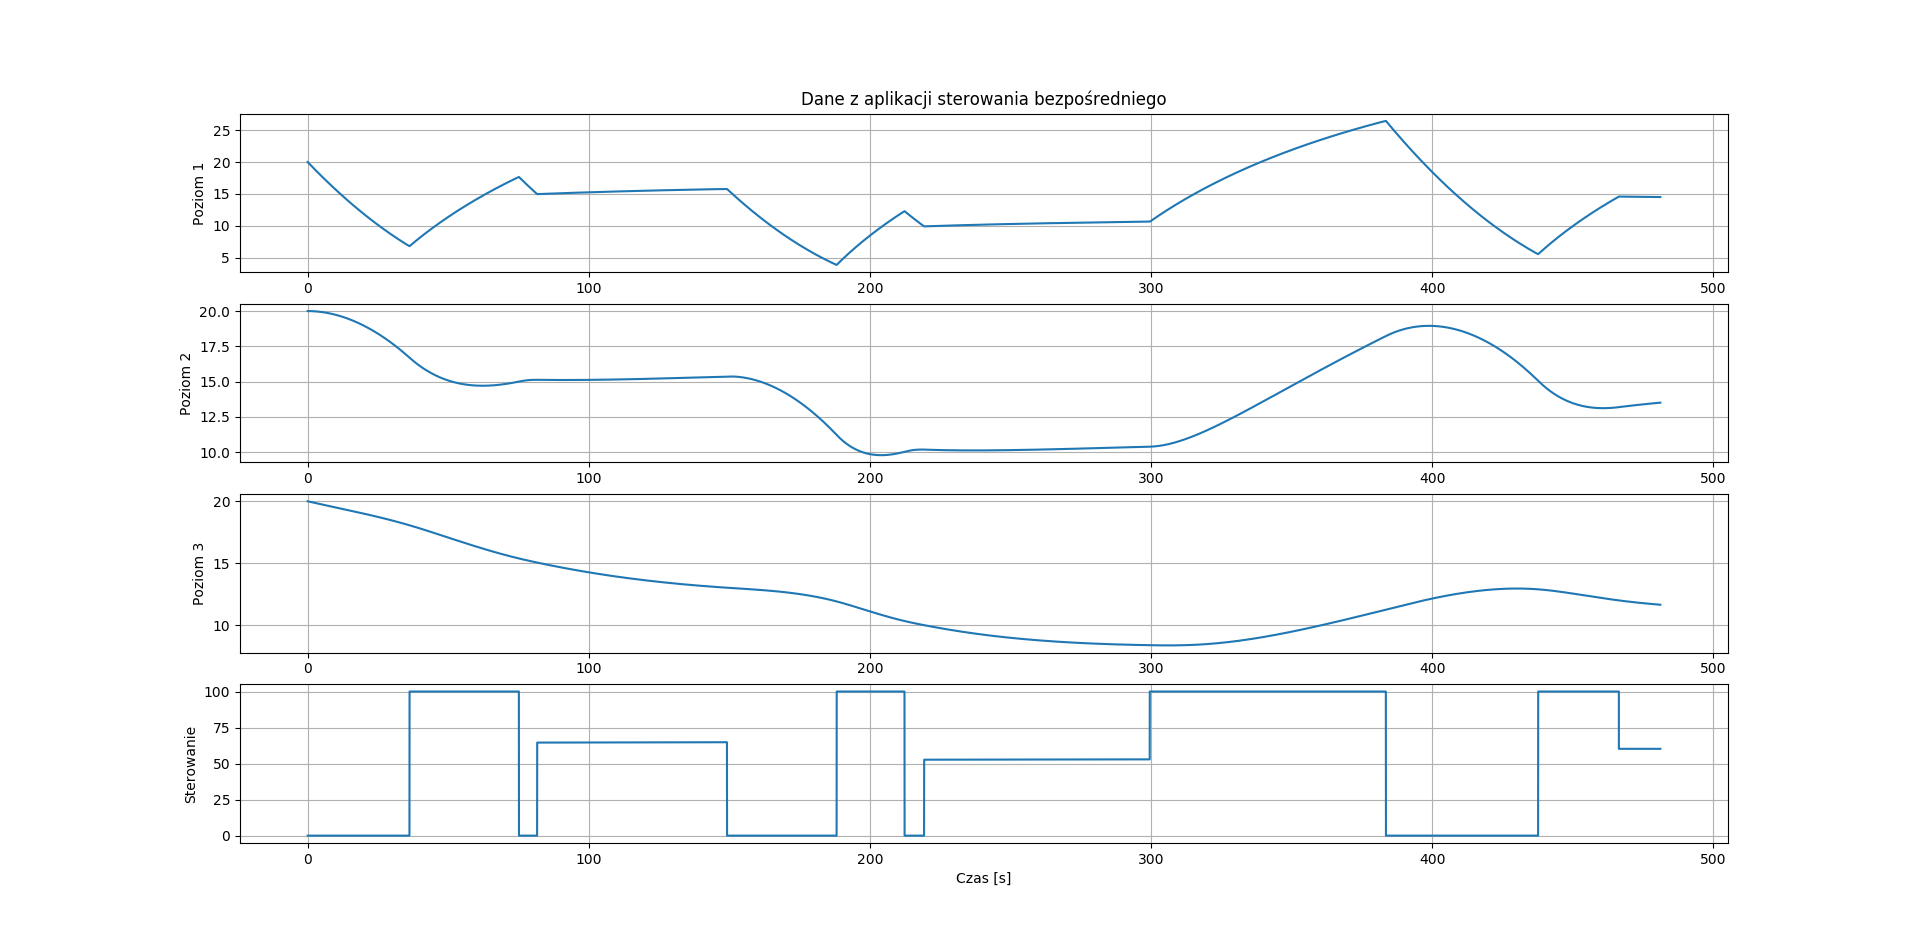
\includegraphics[scale=0.5,angle=90]{Grafika/ext_ctrl_3_opts}
    \caption{Trzy procesy optymalizacji zweryfikowane w symulacji niższego poziomu aplikacji. Źródło: własne.}
    \label{fig:extctrl3opts}
\end{figure}


\begin{table}[htp]
    \centering
    \begin{tabular}{|c|c|c|c|c|}
        \hline 
        \textbf{Czas} & \textbf{Stan początkowy} & \textbf{Stan docelowy} & \textbf{$e_{MATLAB}$} & \textbf{$e_{JModelica.org}$} \\ 
        \hline 
        81,623 & $h^{0} = [20 ~20~ 20]^{T}$ & $h^{f} = [15 ~15~ 15]^{T}$ & 0,021 & 0,008 \\ 
        \hline 
        219,268 & $h^{0} = [15.77~ 15.37~ 13.02]^{T}$ & $h^{f} = [10 ~10~ 10]^{T}$ & 0,047 & 0,0095 \\ 
        \hline 
        466,422 & $h^{0} = [10.62~ 10.39~ 8.37]^{T}$ & $h^{f} = [15 ~13~ 12]^{T}$ & 0,221 & 0,0007 \\ 
        \hline 
    \end{tabular}
\caption{Podsumowanie wyników weryfikacji wyższego i niższego poziomu aplikacji dla trzech optymalizacji przedstawionych na rys. \ref{fig:extctrl3opts}. Źródło: własne.}
\label{tab:extctrl3opts}
\end{table}

\begin{figure}
    \centering
    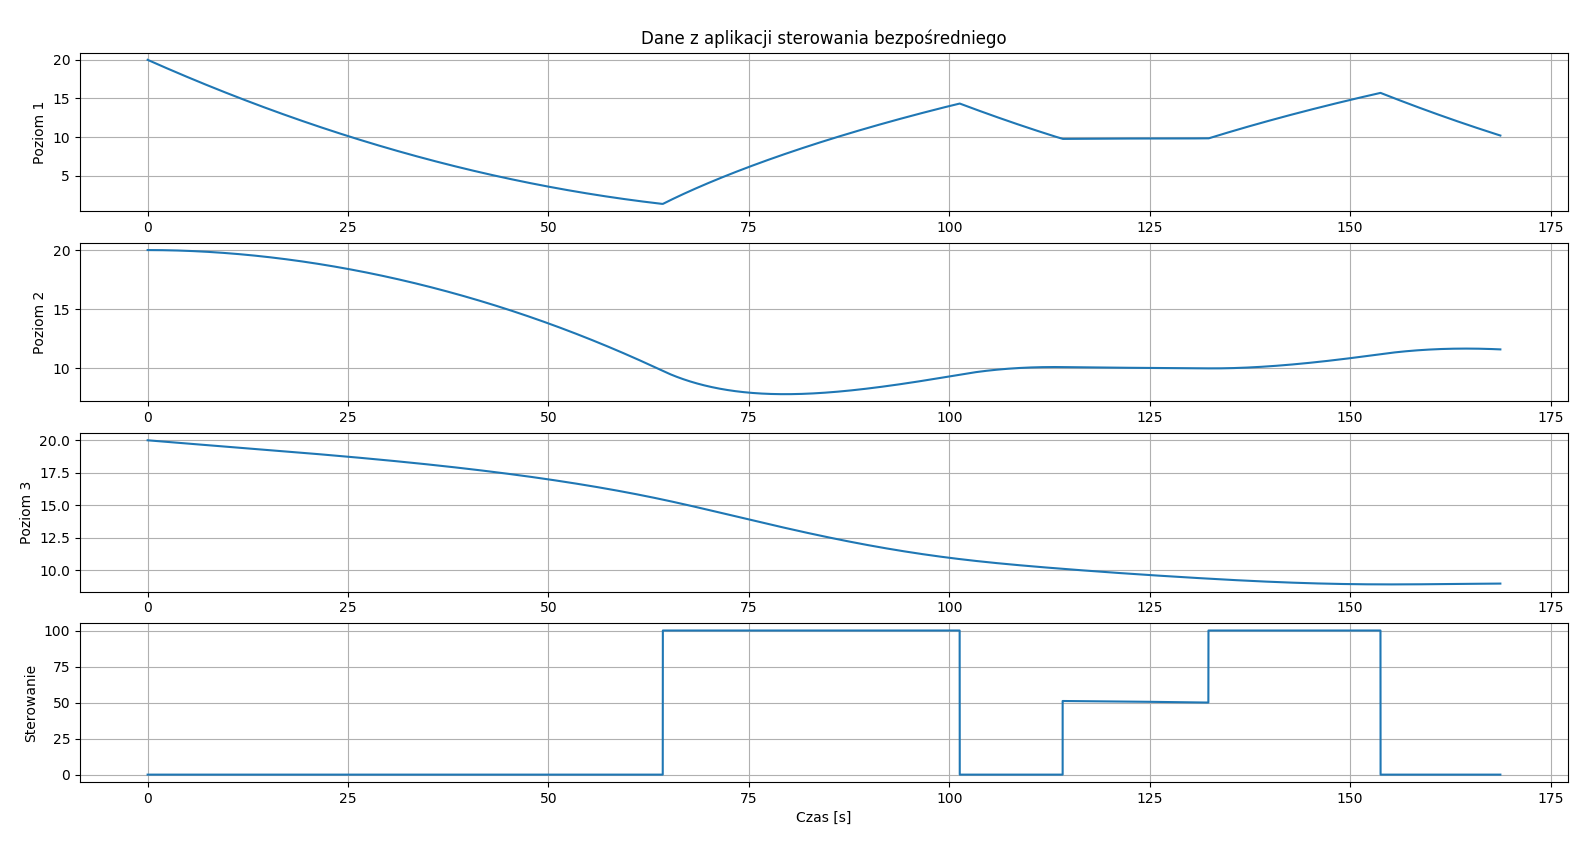
\includegraphics[scale=0.5,angle=90]{Grafika/ext_ctrl_2_opts}
    \caption{Dwa procesy optymalizacji zweryfikowane w symulacji niższym poziomem aplikacji. Źródło: własne.}
    \label{fig:extctrl2opts}
\end{figure}

\begin{table}[htp]
    \centering
    \begin{tabular}{|c|c|c|c|c|}
        \hline 
        \textbf{Czas} & \textbf{Stan początkowy} & \textbf{Stan docelowy} & \textbf{$e_{MATLAB}$} & \textbf{$e_{JModelica.org}$} \\
        \hline 
        114,141 & $h^{0} = [20~ 20~ 20]$ & $h^{f} = [10 ~10~ 10]^{T}$ & 0,081 & 0,002 \\ 
        \hline 
        168,743 & $h^{0} = [9.82~ 9.99~ 9.37]$ & $h^{f} = [10 ~12~ 9]^{T}$ & 0,203 & 0,0005 \\ 
        \hline 
    \end{tabular}
    \caption{Podsumowanie wyników weryfikacji wyższego i niższego poziomu aplikacji dla dwóch optymalizacji przedstawionych na rys. \ref{fig:extctrl2opts}. Źródło: własne.}
    \label{tab:extctrl2opts}
\end{table}

Zauważono, iż błędy weryfikacji na niższym poziomie rosną przy kolejnych optymalizacjach. Dzieje się tak ze względu na fakt, iż aplikacja wyższego poziomu przeprowadza optymalizację na podstawie danych pobranych przed uruchomieniem algorytmu, ale sterowanie jest wysyłane na niższy poziom po zakończeniu jej działania. Przez czas działania algorytmu poziomy zmieniają się jednak i dążą dalej do odpowiedniego punktu równowagi. Ten problem mógłby rozwiązać układ predykcyjny działający po stronie wyższego poziomu aplikacji, który wyznaczałby spodziewane wartości poziomów początkowych w momencie rozpoczęcia aplikacji sterowania czasooptymalnego. Jednakże jak pokazano w sekcji \ref{sub:sym-wer-jmodelica}, czas działania algorytmu optymalizacji jest różny dla różnych zestawów stanów początkowych i końcowych, a jego oszacowanie mogłoby być trudnym zadaniem.

Błędy pierwszych optymalizacji nie powinny być obarczone tym problemem, ale i tak są o rząd wielkości większe od tych uzyskanych na wyższym poziomie aplikacji. Jest to najprawdopodobniej spowodowane niedokładnością wyznaczenia czasów przełączeń: w aplikacji wyższego poziomu do weryfikacji podaje się cały wektor sterowania, a w aplikacji niższego poziomu używa się tylko czasów przełączeń. Mogą grać tu rolę błędy zaokrąglenia i/lub obcięcia


\chapter*{Zakończenie}
\addcontentsline{toc}{chapter}{Zakończenie}
\label{cha:zakonczenie}

Przygotowanie aplikacji realizującej postawione we wstępie niniejszej pracy cele okazało się zadaniem tyleż trudnym, co fascynującym. Obie te cechy wynikały przede wszystkim z założeń postawionych przed wyższym poziomem aplikacji opisanych na początku podrozdziału \ref{sec:czesc-wyzsza}. Znalezienie i opisanie otwartego oprogramowania, które potrafi rozwiązywać problemy optymalizacji dynamicznej układów nieliniowych i posiada przystępny interfejs użytkownika, jest niewątpliwą wartością tej pracy.

Udało się zrealizować wszystkie cele: pokazano, iż wyższy poziom aplikacji jest w stanie wyznaczać sterowanie optymalne w rozumieniu dwóch wskaźników jakości: liniowo-kwadratowego i czasowego. Umożliwia on również przeprowadzenie symulacji weryfikacyjnych wyznaczonych sterowań, które opisano w rozdziale \ref{cha:symulacja}. Niższy poziom aplikacji został przygotowany z myślą o komunikacji z układem pomiarowo-sterującym, ale ona nie została przetestowana. Używano tego poziomu tylko w celach symulacyjnych, co dało możliwość sprawdzenia funkcjonowania wyznaczonego sterowania optymalnego poza środowiskiem, w którym zostało obliczone.

Podstawowym kierunkiem dalszych prac byłoby połączenie napisanej aplikacji z rzeczywistym obiektem, co na pewno dostarczyłyby istotnych wniosków co do funkcjonowania całości aplikacji. Byłoby dobrze uzupełnić również opis problemu o identyfikację elementów wykonawczych oraz wyznaczenie zbioru stanów osiągalnych, aby ograniczyć użytkownikowi zbiór możliwych punktów końcowych optymalizacji. Można by również przygotować układ predykcyjny, w celu poprawy błędów sterowania obliczanego w czasie działania aplikacji. Zapewne byłoby to potrzebne przy użyciu jej z rzeczywistym układem zbiorników.

Poza tym należałoby udoskonalić inicjalizację optymalizacji, gdyż to zagadnienie nie zostało rozpoznane dogłębnie w niniejszej pracy. Jest to jednak problem na tyle złożony, że z powodzeniem mógłby stać się tematem kolejnej pracy dyplomowej. Nie testowano również wszystkich możliwości dostosowania algorytmu optymalizacji do potrzeb tego zagadnienia.


\listoffigures
\addcontentsline{toc}{chapter}{Spis rysunków}

% itd.
% \appendix
% \include{dodatekA}
% \include{dodatekB}
% itd.

\clearpage
\addcontentsline{toc}{chapter}{Bibliografia}
\printbibliography

\end{document}
